\documentclass[11pt]{report}

%to add links but not color
\usepackage{hyperref}
%%Non-ASCII characters
\usepackage[utf8]{inputenc}

%LANGUAGES
\usepackage[spanish,english]{babel}

% Add draft watermark
\usepackage{draftwatermark}
\SetWatermarkScale{3}

%To add frames to verbatim environment
\usepackage{fancyvrb}

\topmargin=-1in    % Make letterhead start about 1 inch from top of page
\textheight=9in  % text height can be bigger for a longer letter
\oddsidemargin=0pt % leftmargin is 1 inch
\textwidth=6.5in   % textwidth of 6.5in leaves 1 inch for right margin
%%\usepackage[hyphens]{url}

%Bib style
\usepackage{natbib}
\bibpunct[: ]{(}{)}{;}{a}{,}{,}

%To Add Figures
\usepackage{graphicx}

\begin{document}
\title{Especificaciones para la anotación de SPinTX\\ con información lingüística para fines pedagógicos}
\author{Martí Quixal}
\date{Diciembre 2012 -- hoy}
\maketitle
\tableofcontents

\cleardoublepage

%%%%%% Final dels agraments
\chapter*{Acknowledgements}
This research is funded by the Longhorn Innovation Fund for Technology (LIFT) for the grant period September 1, 2012 – August 31, 2013.

More information on the Corpus to Classroom website:\\
\url{http://sites.la.utexas.edu/corpus-to-classroom/}

\chapter*{Introducción}
Este documento describe el proceso de anotación de las transcripciones de los clips del corpus SPinTX (Spanish in Texas) con información pedagógica para facilitar el uso de los mismos en la enseñanza y el aprendizaje de español como lengua extranjera.

DOCU
\part{Definición de LIST y SET}
\chapter{LIST y SET basados en información morfosintáctica}
\section{Categorías gramaticales}
\section{Rasgos morfosintácticos}
\chapter{LIST y SET basados en lemas}
\section{Los LIST}
\section{Los SET}
\chapter{LIST y SET basados en palabras (literales)}
\chapter{LIST y SET basados en etiquetas pedagógicas}
\chapter{Definiciones de \emph{templates}}
Los ``templates'' son un tipo de entidad especial en CG3 que sirve para expresar contextos o secuencias de palabras, lemas o etiquetas morfosintácticas que ocurren frecuentemente. 

\part{Secciones previas}
\paragraph*{Rule}
\fbox{
\parbox{.9\linewidth}{\texttt{SUBSTITUTE ("por" Adverb ADV) ("por" Preposition PREP) TARGET ("por");}}
}
\paragraph*{Rule}
\fbox{
\parbox{.9\linewidth}{\texttt{SUBSTITUTE ("por" PDEL) ("por" Preposition PREP) TARGET ("por");}}
}
\chapter{Reglas para rectificar errores del análisis morfosintático}
\paragraph*{Rule}
\fbox{
\parbox{.9\linewidth}{\texttt{SUBSTITUTE (Noun NC Singular Masculine) (Conjunction CCAD) TARGET ("pero");}}
}
\begin{itemize}
\item ETIQ: CC
\item EJEM: \emph{pero} 
\item DESC: Regla para cambiar a \emph{pero} la lectura de nombre por la de conjunción. Ahora se aplica indiscriminadamente, pero podría ser conveniente controlar que antes del pero no hay un artículo. Por ejemplo: ``el pero de la cuestión es que podría romperse el motor''.
\end{itemize}

\paragraph*{Rule}
\fbox{
\parbox{.9\linewidth}{\texttt{SUBSTITUTE ("hecho" Noun NC Singular Masculine) ("hacer" Verb VLadj) TARGET ("hecho") IF (-1 Haber + Verbo);}}
}
\begin{itemize}
\item ETIQ: Cambia Noun NC Singular Masculine por Verb VLadj
\item EJEM: \emph{hecho} 
\item DESC: Regla para cambiar a \emph{pero} la lectura de nombre por la de conjunción. Ahora se aplica indiscriminadamente, pero podría ser conveniente controlar que antes del pero no hay un artículo. Por ejemplo: ``el pero de la cuestión es que podría romperse el motor''.
\end{itemize}

\paragraph*{Rule}
\fbox{
\parbox{.9\linewidth}{\texttt{SUBSTITUTE ("ranchar" Verb VLfin Pres Indi Sing 1st) ("rancho" Noun NC Singular Masculine) TARGET ("ranchar");}}
}
\begin{itemize}
\item ETIQ: Cambia Verb VLfin Pres Indi Sing 1st por Noun NC Singular Masculine en la palabra ``rancho''.
\item EJEM: \emph{rancho} 
\item DESC: Lo hace de forma indiscriminada. Quizá en el futuro habrá que cambiarla, refinarla.
\end{itemize}

\paragraph*{Rule}
\fbox{
\parbox{.9\linewidth}{\texttt{SUBSTITUTE ("dicho" Determiner QU) ("decir" Verbo VLadj) TARGET ("dicho");}}
}
\begin{itemize}
\item ETIQ: Cambia lectura de ``dicho'' como determinante por lectura como adjetivo/participio.
\item EJEM: \emph{dicho} 
\item DESC: Lo hace de forma indiscriminada. Quizá en el futuro habrá que cambiarla, refinarla.
\end{itemize}

\paragraph*{Rule}
\fbox{
\parbox{.9\linewidth}{\texttt{SUBSTITUTE ("oír" Verb VLfin Pres Subj Sing 1st\_or\_3rd) ("oír" Verb VLfin Pres Indi\_Command Sing 2nd\_3rd) TARGET ("oír");}}
}
\begin{itemize}
\item ETIQ: Cambia lectura de "oye" como presente de subjuntivo por lectura de presente de indicativo/imperativo.
\item EJEM: \emph{oye} 
\item DESC: Lo hace de forma indiscriminada. Quizá en el futuro habrá que cambiarla, refinarla.
\end{itemize}

\paragraph*{Rule}
\fbox{
\parbox{.9\linewidth}{\texttt{SUBSTITUTE ("ser" Verb VSfin Pret Indi Plural 3rd) ("ir" Verb VLfin Pret Indi Plural 3rd) TARGET ("<fueron>") IF (-1C SeLiteral);}}
}
\paragraph*{Rule}
\fbox{
\parbox{.9\linewidth}{\texttt{SUBSTITUTE ("ser" Verb VSfin Pret Indi Plural 3rd) ("ir" Verb VLfin Pret Indi Plural 3rd) TARGET ("<fueron>") IF (1 ConLema + Prep);}}
}
\paragraph*{Rule}
\fbox{
\parbox{.9\linewidth}{\texttt{SUBSTITUTE ("ser" Verb VSfin Pret Indi Plural 3rd) ("ir" Verb VLfin Pret Indi Plural 3rd) TARGET ("<fueron>") IF (1 Gerundio);}}
}
\begin{itemize}
\item ETIQ: Reglas que cambian la lectura de "ser" por "ir" en "fueron" cuando no va precedida de un pronombre se o seguida la preposición con o un gerundio.
\item EJEM: \emph{se fueron juntos, se fueron a la escuela} 
\item DESC: Quizá en el futuro habrá que cambiarlas, refinarlas.
\end{itemize}

\paragraph*{Rule}
\fbox{
\parbox{.9\linewidth}{\texttt{SUBSTITUTE ("maestro" Adjective ADJ Singular) ("maestro" Noun Singular) TARGET ("maestro");}}
}
\paragraph*{Rule}
\fbox{
\parbox{.9\linewidth}{\texttt{SUBSTITUTE ("maestro" Adjective ADJ Plural) ("maestro" Noun Plural) TARGET ("maestro");}}
}
\begin{itemize}
\item ETIQ: Cambia lectura de "maestro" de adjetivo sustantivo.
\item EJEM: \emph{maestro, maestra, maestros, maestras} 
\item DESC: Lo hace de forma indiscriminada. Quizá en el futuro habrá que cambiarla, refinarla. Por ejemplo, en "obras maestras", que no ocurre en la versión actal del corpus.
\end{itemize}

\paragraph*{Rule}
\fbox{
\parbox{.9\linewidth}{\texttt{SUBSTITUTE ("erar|ser" Verb VLfin Past Subj Sing 2nd) ("ser" Verb VSfin Imp Indi Sing 2nd) TARGET ErasLiteral;}}
}
\paragraph*{Rule}
\fbox{
\parbox{.9\linewidth}{\texttt{SUBSTITUTE ("erar|ser" Verb VLfin Past Subj Plural 2nd\_or\_3rd) ("ser" Verb VSfin Imp Indi Plural 3rd) TARGET EranLiteral;}}
}
\paragraph*{Rule}
\fbox{
\parbox{.9\linewidth}{\texttt{SUBSTITUTE ("UNK" Noun NC) ("ser" Verb VSfin Imp Indi Sing 1st\_or\_3rd) TARGET EraMayusLiteral;}}
}
\begin{itemize}
\item ETIQ: Cambia lectura de "eras" y "eran" de lema ambiguo entre erar y ser a sólo lema ser.
\item EJEM: \emph{eras, eran} 
\item DESC: Consideramos erar un verbo muy poco frecuente. Si hiciera falta, se podría refinar la regla.
\end{itemize}

\paragraph*{Rule}
\fbox{
\parbox{.9\linewidth}{\texttt{SUBSTITUTE ("UNK" Noun NC Plural) ("mío" Pronoun PPO Plural) TARGET ("<mis>") OR ("<Mis>");}}
}
\paragraph*{Rule}
\fbox{
\parbox{.9\linewidth}{\texttt{SUBSTITUTE ("UNK" Noun NC Plural) ("nuestro" Pronoun PPO Plural) TARGET ("<nuestros>") OR ("<Nuestros>");}}
}
\begin{itemize}
\item ETIQ: Cambia lectura de "UNK" Noun NC Plural a "mío" Pronoun PPO Plural a "mis".
\item EJEM: \emph{mis,Mis} 
\item DESC: Lo hacemos con nuestros (y quizás habrá que añadir otros posesivos).
\end{itemize}

\paragraph*{Rule}
\fbox{
\parbox{.9\linewidth}{\texttt{SUBSTITUTE ("dar|decir" Verb VLfin Pres Command Sing 2nd) ("dar" Verb VLfin Pret Indi Sing 1st) TARGET DiLiteral IF (-1 PronombresCliticosTODOS);}}
}
\begin{itemize}
\item ETIQ: Cambia lectura de "di" de lema ambiguo entre dar y decir a sólo lema dar.
\item EJEM: \emph{le di, me di cuenta} 
\item DESC: Dado que ``di'' como mandato llevará siempre el clítico pospuesto, si no lo lleva lo podemos considerar una forma de dar. Cabría tener en cuenta otras opciones pero esta parece razonable.
\end{itemize}

\paragraph*{Rule}
\fbox{
\parbox{.9\linewidth}{\texttt{SUBSTITUTE (Verb VLinf Pres Command Plural 2nd) (Verb VLinf) TARGET ("<(.*)(ar|er|ir|ír)>"r); }}
}
\begin{itemize}
\item ETIQ: Cambia lectura Command Plural 2nd a los infinitivos marcados como imperativo (y que estrictamente no los son)
\item EJEM: \emph{decir, nadar, temer} 
\item DESC: Se aplica a cualquier infinitivo con la lectura arriba mencionada. A pesar de que los imperativos pueden tener esta función de mandatopragmáticamente hablando, consideramos que no se deben etiquetar morfológicamente como tales.
\end{itemize}

OBSERVACIÓN: Notad la ``r'' al final del TARGET en la regla. Indica que lo anterior debe ser tratado como una expresión regular. Si no, la regla no se aplica.

\paragraph*{Rule}
\fbox{
\parbox{.9\linewidth}{\texttt{SUBSTITUTE ("UNK" Verb VLfin Pres Command Plural 2nd) ("platicar" Verb VLfin Pres Command Sing 3rd) TARGET ("<platíquenos>");}}
}
\begin{itemize}
\item ETIQ: Cambia lectura Command Plural 2nd y lema a ``platíquenos'' 
\item EJEM: \emph{platíquenos} 
\item DESC: Se aplica sólo a ``platíquenos''.
\end{itemize}

\paragraph*{Rule}
\fbox{
\parbox{.9\linewidth}{\texttt{SUBSTITUTE ("tener" Verb VMfin) ("tener" Verb VMfin Past Subj Plural 3rd) TARGET ("<tengan>");}}
}
\begin{itemize}
\item ETIQ: Añade lectura de pasado de subjuntivo a tener cuando este recibe el tag VMFin. 
\item EJEM: \emph{tengan} 
\item DESC: Se aplica sólo a ``tengan''.
\end{itemize}

\paragraph*{Rule}
\fbox{
\parbox{.9\linewidth}{\texttt{SUBSTITUTE ("para" Conjunction CSUBI) ("para" Preposition PREP) TARGET ("para");}}
}
\begin{itemize}
\item ETIQ: Cambia la lectura de conjunción de subordinación de infinitivas por la de preposición. 
\item EJEM: \emph{tengan} 
\item DESC: Se aplica sólo a ``para'' como lema.
\end{itemize}

OBSERVACIÓN: Aunque es verdad que ``para'' puede ir seguida de un infinitivo para formar una subordinada infinitiva esta es una función que pueden desempeñar otras preposiciones, y creo que no por ello hay que cambiarles su categoría gramatical principal.

\paragraph*{Rule}
\fbox{
\parbox{.9\linewidth}{\texttt{SUBSTITUTE ("crear" Verb VLfin Past Subj Plural 3rd) ("creer" Verb VLfin Pres Indi Plural 3rd) TARGET ("<creen>") IF (1 LoLiteral) (2 MismoLiteral) (3 Que);}}
}
\paragraph*{Rule}
\fbox{
\parbox{.9\linewidth}{\texttt{SUBSTITUTE ("crear" Verb VLfin Past Subj Plural 3rd) ("creer" Verb VLfin Pres Indi Plural 3rd) TARGET ("<creen>") IF (1 En OR Que);}}
}
\paragraph*{Rule}
\fbox{
\parbox{.9\linewidth}{\texttt{SUBSTITUTE ("crear" Verb VLfin Past Subj Plural 3rd) ("creer" Verb VLfin Pres Indi Plural 3rd) TARGET ("<creen>")  IF (-2 NoAdv) (-1 PronombresCliticosTODOS OR SeLiteral);}}
}
\begin{itemize}
\item ETIQ: Varias reglas para dar la lectura indicativa de ``creer'' a la forma ``creen'' en lugar de la subjuntiva de ``crear''. 
\item EJEM: \emph{tengan} 
\item DESC: Se aplica teniendo en cuenta algunos contextos que generalmente decantaran la lectura hacia la interpretación prevista (creer).
\end{itemize}

\paragraph*{Rule}
\fbox{
\parbox{.9\linewidth}{\texttt{SUBSTITUTE ("UNK" Noun NC Plural) ("bueno" Adjective ADJ Plural Masc) TARGET ("<Buenos>");}}
}
\paragraph*{Rule}
\fbox{
\parbox{.9\linewidth}{\texttt{SUBSTITUTE ("cierta|cierto" Determiner QU) ("cierta|cierto" Determiner QU Plural Fem) TARGET ("<ciertas>") OR ("<Ciertas>");}}
}
\paragraph*{Rule}
\fbox{
\parbox{.9\linewidth}{\texttt{SUBSTITUTE ("cierta|cierto" Determiner QU) ("cierta|cierto" Determiner QU Singular Fem) TARGET ("<cierta>") OR ("<Cierta>");}}
}
\begin{itemize}
\item ETIQ: Reglas para dar a cierta(s) el lema cierto. El lema cierta no se corresponde con ninguna lectura documentada en los diccionarios de referencia (RAE o DEM). 
\item EJEM: \emph{cierta}, \emph{cierta}
\item DESC: NA.
\end{itemize}

\paragraph*{Rule}
\fbox{
\parbox{.9\linewidth}{\texttt{SUBSTITUTE ("cuarto" Determiner QU) ("cuarto" Noun NC Singular Masc) TARGET ("<cuarto>") OR ("<Cuarto>") IF (NOT 1 Nombre);}}
}
\paragraph*{Rule}
\fbox{
\parbox{.9\linewidth}{\texttt{SUBSTITUTE ("cuarto" Determiner QU) ("cuarto" Adjective ORD Singular Masc) TARGET ("<cuarto>") OR ("<Cuarto>") IF (1C Nombre + SG);}}
}
\begin{itemize}
\item ETIQ: For some reason TreeTagger tags cuarto as DetQU. I assume this is because they include cardinals in this category, which is a very arguable decision in my opinion. I decided to change it to either noun or adjective depending on the contexts. 
\item EJEM: (...) nosotras teníamos que compartir nuestros, nuestro \emph{cuarto}, teníamos tres niñas por cuarto (...)  (Noun)
\item EJEM: (...) ellos eran, los paraguayitos eran de \emph{cuarto} grado. (Adjective)
\item DESC: NA.
\end{itemize}

\paragraph*{Rule}
\fbox{
\parbox{.9\linewidth}{\texttt{SUBSTITUTE ("doble" Determiner QU) ("doble" Adjective ADJ Singular Masc-Fem) TARGET ("<doble>") OR ("<Doble>");}}
}
\begin{itemize}
\item ETIQ: Contrary to TreeTagger RAE and most standard sources of Spanish linguistics think that doble is an adjective, even if it can be modifying a noun as some determiners can. For this, I decided to change its reading to adjective depending always. 
\item EJEM: (...) \emph{doble}
\item DESC: NA.
\end{itemize}

\paragraph*{Rule}
\fbox{
\parbox{.9\linewidth}{\texttt{SUBSTITUTE ("ambo" Determiner QU) ("ambos" Determiner QU Plural Masc) TARGET ("<ambos>") OR ("<Ambos>");}}
}
\paragraph*{Rule}
\fbox{
\parbox{.9\linewidth}{\texttt{SUBSTITUTE ("ambo" Determiner QU) ("ambos" Determiner QU Plural Fem) TARGET ("<ambas>") OR ("<Ambas>");}}
}
\begin{itemize}
\item ETIQ: TreeTagger assignes lemma ambo to determiner ambos. The word ambo exists, but it has nothing to do (nowadays) with the determiner ambos/ambas. It will always be handled as a determiner. 
\item EJEM: (...) \emph{ambos}, \emph{ambas} ...
\item DESC: NA.
\end{itemize}

\paragraph*{Rule}
\fbox{
\parbox{.9\linewidth}{\texttt{SUBSTITUTE ("poco" Noun NC) ("poco" Adverb ADV) TARGET ("<poquito>") OR ("<POQUITO>") IF (NOT -1 UnDetLiteral);}}
}
\paragraph*{Rule}
\fbox{
\parbox{.9\linewidth}{\texttt{SUBSTITUTE ("poco" Noun NC) ("poco" Adjective ADJ Singular Masc) TARGET ("<poquito>") OR ("<POQUITO>") IF (-1 UnDetLiteral);}}
}
\begin{itemize}
\item ETIQ: TreeTagger asigna la lectura nominal a poco en algunos contextos en que consideramos que debería ser adverbio o adjectivo. Estas reglas lo tratan.
\item EJEM: (...) \emph{ambos}, \emph{ambas} ...
\item DESC: NA.
\end{itemize}

\paragraph*{Rule}
\fbox{
\parbox{.9\linewidth}{\texttt{SUBSTITUTE ("y" Other ALFS) ("y" Conjunciton CC) TARGET ("<y>") OR ("<Y>");}}
}
\paragraph*{Rule}
\fbox{
\parbox{.9\linewidth}{\texttt{SUBSTITUTE ("Y" Other ALFS) ("y" Conjunciton CC) TARGET ("<y>") OR ("<Y>");}}
}
\paragraph*{Rule}
\fbox{
\parbox{.9\linewidth}{\texttt{SUBSTITUTE ("o" Other ALFS) ("o" Conjunciton CC) TARGET ("<o>") OR ("<O>");}}
}
\paragraph*{Rule}
\fbox{
\parbox{.9\linewidth}{\texttt{SUBSTITUTE ("O" Other ALFS) ("o" Conjunciton CC) TARGET ("<o>") OR ("<O>");}}
}
\paragraph*{Rule}
\fbox{
\parbox{.9\linewidth}{\texttt{SUBSTITUTE ("a" Other ALFS) ("a" Preposition PREP) TARGET ("<a>") OR ("<A>") (NOT 1 PalabraEnIngles);}}
}
\begin{itemize}
\item ETIQ: TreeTagger asigna la lectura ALFS a palabras como ``y'', ``o'' o ``a''. Estas reglas lo reparan.
\item EJEM: (...) \emph{y}, \emph{o}, \emph{a} ...
\item DESC: Todavía quedan algunas letras sueltas que reciben esta etiqueta, pero no he seguido trabajando en ello porque son un número absoluto y relativo bastante bajo.
\end{itemize}

\paragraph*{Rule}
\fbox{
\parbox{.9\linewidth}{\texttt{SUBSTITUTE ("medio" Preposition PDEL) ("medio" Noun NC Singular Masc) TARGET MedioLiteral IF (-1 PorLiteral) (1 PrepContract);}}
}
\paragraph*{Rule}
\fbox{
\parbox{.9\linewidth}{\texttt{SUBSTITUTE ("medio" Adjective ADJ) ("medio" Determiner QU Singular Masc) TARGET MedioLiteral IF (1C Adj);}}
}
\paragraph*{Rule}
\fbox{
\parbox{.9\linewidth}{\texttt{SUBSTITUTE ("medio" Noun NC Singular) ("medio" Determiner QU Singular Masc) TARGET MedioLiteral IF (0C MedioLiteral) (NOT 0 DetQU) (*-2 DetCardinales OR UnDetLiteral BARRIER FiniteVerbForms OR Conjuncion OR LimiteOracionSimple) (-1 YLiteral);}}
}
\begin{itemize}
\item ETIQ: Pasa de PDEL a NC a ``medio''. O de NC a QU, según los contextos.
\item EJEM: (...) \emph{un año y medio}, lo hice \emph{por medio de} su hermana ...
\item DESC: TreeTagger asigna lecturas curiosas a ``medio''. Entre ellas PDEL en ``por medio de'' o nombre en expresiones como ``un año y medio''. Escribo un pare de reglas para cambiar esto, pero la verdad es que medio es una de esas palabras complicadas a la que cabría prestar atención (junto con el resto de determinantes y los llamados adjetivos pronominales, porque tiene un comportamiento peculiar).
\end{itemize}

\paragraph*{Rule}
\fbox{
\parbox{.9\linewidth}{\texttt{SUBSTITUTE ("material" Adjective ADJ Plural) ("material" Noun NC Plural Masc) TARGET ("<materiales>"i) IF (-1 DetAllIncluded) (1 Adj + PL);}}
}
\begin{itemize}
\item ETIQ: Asigna lectura Noun a ``materiales'' en lugar de la adjetivo.
\item EJEM: (...) \emph{un año y medio}, lo hice \emph{por medio de} su hermana ...
\item DESC: En contextos en que materiales va precedido por un determinante y seguido de un Adjetivo en plural.
\end{itemize}

\paragraph*{Rule}
\fbox{
\parbox{.9\linewidth}{\texttt{SUBSTITUTE ("gracias" Preposition PREP) ("gracia" Noun NC Plural Fem) TARGET ("<gracias>"i);}}
}
\begin{itemize}
\item ETIQ: Asigna lectura Noun a ``gracias'' incluso si format parte de la locución ``gracias a''.
\item EJEM: \emph{gracias a} Dios, \emph{gracias a} la tecnología
\item DESC: Que la locución ``gracias a'' sea prepositiva (o preposicional) no signigica que sus elementos sean todos preposiciones. Esto va contra las reglas de composición de expresiones (lexicalizadas o no) del lenguaje.
\end{itemize}

\paragraph*{Rule}
\fbox{
\parbox{.9\linewidth}{\texttt{SUBSTITUTE ("decir" Verb VLfin Pres Indi Sing 1st) ("decir" Verb VLfin Pret Indi Sing 3rd) TARGET ("<dijo>"i);}}
}
\begin{itemize}
\item ETIQ: Asigna lectura de pretérito perfecto en 3a persona a dijo (que originalmente viene como presente de la 1a persona).
\item EJEM: \emph{dijo}
\item DESC: NA.
\end{itemize}

\paragraph*{Rule}
\fbox{
\parbox{.9\linewidth}{\texttt{SUBSTITUTE ("crear|creer" Verb VLfin Pres Indi Sing 2nd) ("creer" Verb VLfin Pres Indi Sing 2nd) TARGET ("<crees>"i) IF (1 Que);}}
}
\begin{itemize}
\item ETIQ: Desambiguar el lema de ``crees'' para `creer' y o `crear'.
\item EJEM: \emph{crees}
\item DESC: Seguido de un `que'.
\end{itemize}

\paragraph*{Rule}
\fbox{
\parbox{.9\linewidth}{\texttt{SUBSTITUTE ("en" Adverb ADV) ("en" Preposition PREP) TARGET ("<en>"i);}}
}
\begin{itemize}
\item ETIQ: Asignar siempre PREP a ``en'' aunque forme parte de una locución.
\item EJEM: \emph{en}
\item DESC: NA.
\end{itemize}

\paragraph*{Rule}
\fbox{
\parbox{.9\linewidth}{\texttt{SUBSTITUTE ("realidad" Adverb ADV) ("realidad" Noun NC Singular Fem) TARGET ("<realidad>"i);}}
}
\begin{itemize}
\item ETIQ: Asignar siempre Noun a ``realidad'' aunque forme parte de una locución.
\item EJEM: \emph{realidad}
\item DESC: NA.
\end{itemize}

\paragraph*{Rule}
\fbox{
\parbox{.9\linewidth}{\texttt{SUBSTITUTE ("afuera" Noun NP Singular) ("afuera" Adverb ADV) TARGET ("<afuera>"i);}}
}
\begin{itemize}
\item ETIQ: Asignar siempre ADV a ``afuera''.
\item EJEM: \emph{afuera}
\item DESC: NA.
\end{itemize}

\paragraph*{Rule}
\fbox{
\parbox{.9\linewidth}{\texttt{SUBSTITUTE ("UNK" Adjective ADJ Singular) ("chistoso" Adjective ADJ Singular Fem) TARGET ("<chistosa>"i);}}
}
\paragraph*{Rule}
\fbox{
\parbox{.9\linewidth}{\texttt{SUBSTITUTE ("UNK" Adjective ADJ Plural) ("chistoso" Adjective ADJ Plural Fem) TARGET ("<chistosas>"i);}}
}
\paragraph*{Rule}
\fbox{
\parbox{.9\linewidth}{\texttt{SUBSTITUTE ("UNK" Adjective ADJ Plural) ("chistoso" Adjective ADJ Plural Masc) TARGET ("<chistosos>"i);}}
}
\begin{itemize}
\item ETIQ: Asignar lema y rasgos morfosintácticos a las formas marcadas de chistoso.
\item EJEM: \emph{chistosa, chistosas, chistosos}
\item DESC: NA.
\end{itemize}

\part{Secciones principales}
Las reglas de identificación de fenómenmos pedagógicos están ordenadas de más concretas a más generales. Así, por ejemplo, se detectan primero, cuando es posible, los distintos usos de \emph{para} (opinión, intención, destino, etc. como \emph{@Gram:Prep:Para:Opinion}...) y luego se marcan como simplemente \emph{@Gram:Prep:Para} el resto de ocurrencias de \emph{para}. Luego, se hace lo propio con otras preposiciones, hasta el punto que si para una preposición no hay reglas especiales, sus ocurrencias se marcan simplemente como \emph{@Gram:Prep}.

Esta estrategia se utiliza para evitar que una misma palabra reciba por partida doble informaciones de igual granularidad. Para ello, antes de asignar una etiqueta, se comprueba que no haya otra asignada del mismo nivel. A efectos prácticos, etiquetas como \emph{@Gram:Prep:Para:Opinion}...) y \emph{@Gram:Prep:Para} se consideran del mismo nivel.

Para evitar este tipo de duplicidades también se podría usar una estrategia basada en la distinción entre ADD y MAP (véase la documentación de vislcg3). Por ahora no se ha hecho, porque esto impide la asignación de múltiples etiquetas a un mismo token/una misma palabra.

REM: Ahora mismo sólo estamos asignando hasta tres niveles de descripción pedagógica. Veáse el Google Doc Pedagogical tipologies \url{https://docs.google.com/spreadsheet/ccc?key=0AlyBsKogCRnwdDd3ZWRjejZlQU5XZWl6WVVUZmtKcEE&usp=sharing}.
\chapter{Uso de los determinantes}
\section{Usos de los artículos definidos}
Identificaremos los usos de los artículos definidos \emph{el, la, los, las}, y el artículo (en algunas gramáticas considerado pronombre) \emph{lo} cuando va seguido de un adjetivo.

\paragraph*{Rule}
\fbox{
\parbox{.9\linewidth}{\texttt{ADD (@Gram:Det:Art) Articulo IF (0 DetArtDefinidosLiterales) (NOT 1 FiniteVerbForms OR PronombreDeObjetoNoAmbiguos OR SeLiteral);}}
}
\begin{itemize}
\item ETIQ: Asigna @Gram:Det:Art
\item EJEM: \emph{el, la, los, las}
\item DESC: Cualquier ocurrencia no seguida de un verbo finito o un pronombre clítico, porque treetagger no distingue entre su lectura como determinante y la pronominal.
\end{itemize}

\paragraph*{Rule}
\fbox{
\parbox{.9\linewidth}{\texttt{ADDRELATION (Gram:Det:LoAdj) Articulo IF (0 LoLiteral) TO (*1 Adj BARRIER FiniteVerbForms OR Conjuncion OR LimiteOracionSimple LINK NOT 0 MejorLiteral) ;}}
}
\paragraph*{Rule}
\fbox{
\parbox{.9\linewidth}{\texttt{ADDRELATION (Gram:Det:LoAdj) Articulo IF (0 LoLiteral) TO (1 Que) ;}}
}
\paragraph*{Rule}
\fbox{
\parbox{.9\linewidth}{\texttt{ADDRELATION (Gram:Det:LoAdj) Articulo IF (0 LoLiteral) TO (*2 Que BARRIER FiniteVerbForms OR Conjuncion OR LimiteOracionSimple LINK -1 Adj + SG OR Adverbio OR DetQU + SG LINK NOT 0 LemasQueNoSonDetQUStandard) ;}}
}
\begin{itemize}
\item ETIQ: Asigna R:Gram:Det:Art
\item EJEM: \emph{lo} + ADJETIVO 
\item EJEM: \emph{lo} que 
\item EJEM: \emph{lo} poco/importante/mucho que 
\item DESC: Cualquier ocurrencia de LO seguida de un adjetivo o de un que. Puede haber un adverbio intercalado. Quizás habrá que refinar la regla algún día. No anota ``a lo mejor'', ya que esta locución se usa más frecuentement en el sentido de quizás (por los menos en SPinTX).
\end{itemize}

\section{Usos de los determinantes demostrativos}
\paragraph*{Rule}
\fbox{
\parbox{.9\linewidth}{\texttt{ADD (@Gram:Det:Demo) ArtPronDemo IF (-1 Prep OR FiniteVerbForms) (0 EsteEseAquel) (NOT 0 EstoEsoAquello) (1 Nombre) ;}}
}
\begin{itemize}
\item ETIQ: Asigna @Gram:Det:Demo
\item EJEM: Prep/Verbo \emph{este/ese/aquel} (LEMMA) + Nombre
\item DESC: Cualquier ocurrencia de un demostrativo precedida de una preposición o un verbo conjugado y seguido de un nombre.
\end{itemize}

\section{Usos pronominales de los demostrativos}
\paragraph*{Rule}
\fbox{
\parbox{.9\linewidth}{\texttt{ADD (@Gram:Det:Demo) ArtPronDemo IF (-1 Prep OR FiniteVerbForms) (0 EstoEsoAquello) ;}}
}
\begin{itemize}
\item ETIQ: Asigna @Gram:Pron:Demo
\item EJEM: Prep/Verbo \emph{esto/eso/aquello}
\item DESC: Cualquier ocurrencia de un demostrativo terminado en -o. No distinguimos las formas que forman parte de locuciones (como ``por eso'', etc.).
\end{itemize}

\section{Usos de los determinantes posesivos}
\paragraph*{Rule}
\fbox{
\parbox{.9\linewidth}{\texttt{ADD (@Gram:Det:Pos) DetPosSing IF (*1 Nombre + SG BARRIER FiniteVerbForms OR Conjuncion OR LimiteOracionSimple) ;}}
}
\paragraph*{Rule}
\fbox{
\parbox{.9\linewidth}{\texttt{ADD (@Gram:Det:Pos) DetPosPlu IF (*1 Nombre + PL BARRIER FiniteVerbForms OR Conjuncion OR LimiteOracionSimple) ;}}
}
\paragraph*{Rule}
\fbox{
\parbox{.9\linewidth}{\texttt{ADD (@Gram:Det:Pos) DetPosFemPlu IF (*1 Nombre + PL BARRIER FiniteVerbForms OR Conjuncion OR LimiteOracionSimple) ;}}
}
\paragraph*{Rule}
\fbox{
\parbox{.9\linewidth}{\texttt{ADD (@Gram:Det:Pos) DetPosMascPlu IF (*1 Nombre + PL BARRIER FiniteVerbForms OR Conjuncion OR LimiteOracionSimple) ;}}
}
\paragraph*{Rule}
\fbox{
\parbox{.9\linewidth}{\texttt{ADD (@Gram:Det:Pos) DetPosFemSing IF (*1 Nombre + SG BARRIER FiniteVerbForms OR Conjuncion OR LimiteOracionSimple) ;}}
}
\paragraph*{Rule}
\fbox{
\parbox{.9\linewidth}{\texttt{ADD (@Gram:Det:Pos) DetPosMascSing IF (*1 Nombre + SG BARRIER FiniteVerbForms OR Conjuncion OR LimiteOracionSimple) ;}}
}
\begin{itemize}
\item ETIQ: Asigna @Gram:Det:Poss
\item EJEM: Prep/Verbo \emph{mi/tu/su/sus/nuestro/nuestros/vuestro/vuestros} (LEMMA) + Nombre
\item DESC: Cualquier ocurrencia de un determinante posesivo seguido de un nombre (se admiten ADV y ADJ intercalados).
\end{itemize}

\section{Usos de los determinantes indefinidos}
\paragraph*{Rule}
\fbox{
\parbox{.9\linewidth}{\texttt{ADD (@Gram:Det:CuantIndef) UnoLiteral IF (1 De) (NOT -1 Infinitive);}}
}
\begin{itemize}
\item ETIQ: Asigna @Gram:Det:CuantIndef
\item EJEM: Que no los puedo criticar porque yo soy \emph{uno} de ellos (...)
\item DESC: Cualquier ocurrencia de un determinante posesivo seguido de un nombre (se admiten ADV y ADJ intercalados).
\end{itemize}

\paragraph*{Rule}
\fbox{
\parbox{.9\linewidth}{\texttt{ADD (@Gram:Det:CuantIndef) DetQU IF (0 ListaDeDeterminantesSeguros) (NOT 0 NingunoLiteral);}}
}
\begin{itemize}
\item ETIQ: Asigna @Gram:Det:CuantIndef
\item EJEM: (...) porque él vivía aquí , en El Paso e iba \emph{cada} ocho días.
\item DESC: Se aplica a cualquier ocurrencia de determinantes cuantitativos o indefinidos que consideramos ``seguros'' en el sentido de que no tienen intepretación adverbial: ``cualquier'', ``cada'', ``ambos'', ``alguno'', ``tal'' o ``ningún''.
\end{itemize}

\paragraph*{Rule}
\fbox{
\parbox{.9\linewidth}{\texttt{ADD (@Gram:Det:CuantIndef) DetQU IF (0 ("<(.*)(os|as|a)>"r) + ListaDeDeterminantesSegurosSiNoEstanEnMasc) (NOT -1 DetAllIncluded);}}
}
\begin{itemize}
\item ETIQ: Asigna @Gram:Det:CuantIndef
\item EJEM: (...) éramos \emph{muchos} primos y fue muy una experiencia bonita.
\item DESC: Se aplica a cualquier ocurrencia de determinantes cuantitativos o indefinidos que consideramos ``seguros'' en femenino, masculino plural o femenino plural. En masculino singular pueden tener lectura adverbial y por ello proponemos tratarlos a parte (con otro conjunto de reglas, pero con el mimsmo etiquetaje). Ejemplos: ``mucho'', ``poco'', ``tanto'', ``demasiado'', ``cierto'', ``varios'', y ``diversos''. A pesar de que TreeTagger etiqueta  ``dicho'' como determinante en algunos contextos, nosotros lo corregimos a posteriori y lo etiquetamos siempre como participio.
\end{itemize}

\paragraph*{Rule}
\fbox{
\parbox{.9\linewidth}{\texttt{ADD (@Gram:Det:Pron) DetQU IF (0 AlgoLema) (NOT 1 Adj OR AdvIntensificadorAdjetivos);}}
}
\paragraph*{Rule}
\fbox{
\parbox{.9\linewidth}{\texttt{ADD (@Gram:Det:Pron) DetQU IF (0 NadaLema) (NOT 1 Adj OR AdvIntensificadorAdjetivos);}}
}
\paragraph*{Rule}
\fbox{
\parbox{.9\linewidth}{\texttt{ADD (@Gram:Det:Pron) DetQU IF (0 AlgoLema OR NadaLema) (1C Adj);}}
}
\begin{itemize}
\item ETIQ: Asigna @Gram:Det:Pron
 E: 
\item DESC: Se aplica a varios usos de ``nada'' y ``algo'', que demuestran que tiene un comportamiento esencialmente pronominal, porque nunca pueden aparecer modificando a un sustantivo.
\end{itemize}

\paragraph*{Rule}
\fbox{
\parbox{.9\linewidth}{\texttt{ADDRELATION (Gram:Det:Combi) (Determiner) IF (0 DetAllIncluded) TO (1 ListaDeDeterminantesSegurosSiNoEstanEnMasc OR DemasLiteral OR OtroLema LINK NOT 0 Adverbio);}}
}
\begin{itemize}
\item ETIQ: Asigna @Gram:Det:Combi
\item EJEM: (...) \emph{las demás} mamás que estaban fuera, eran como si fueran nuestras propias madres.
\item DESC: Se aplica sobre combinaciones de determinantes
\end{itemize}

\paragraph*{Rule}
\fbox{
\parbox{.9\linewidth}{\texttt{ADDRELATION (Gram:Det:Combi) (Determiner) IF (0 TodosYTodasLiteral OR TodoYTodaLiteral) TO (1 DetAllIncluded);}}
}
\begin{itemize}
\item ETIQ: Asigna @Gram:Det:Combi
\item EJEM: Mi papá mudaba todas las cosas, \emph{todos los} muebles los ponía en el barco (...)
\item DESC: Se aplica sobre combinaciones de determinantes
\end{itemize}

\paragraph*{Rule}
\fbox{
\parbox{.9\linewidth}{\texttt{ADD (@Gram:Det:TodoEsp) (Determiner) IF (0 Todo) (NOT 1 DetAllIncludedNoPosPlural OR Prep OR FiniteVerbForms OR Adverbio OR LimiteOracionSimple OR Puntuacion OR SeLiteral);}}
}
\begin{itemize}
\item ETIQ: Asigna @Gram:Det:TodoEsp
 E: 
\item DESC: No se aplica si va seguido de determinante, verbo conjugado o preposición porque entonces se trata de otro tipo de uso (seguramente el pronominal, como en ``se quebró todo'' o el pre-especificador, como en ``se comió todo el arroz'')
\end{itemize}

\chapter{Género gramatical y artículos}
\section{Género masculino en palabras terminadas en ``a''}
\paragraph*{Rule}
\fbox{
\parbox{.9\linewidth}{\texttt{ADDRELATION (Gram:Genero:ExcepMasc) DetAllIncluded IF (0 ElDetLiteral + SG OR UnDetLiteral + SG OR ArtPronDemo + SG) TO (1 SustMascAcabadosEnA + Nombre + SG) ;}}
}
\begin{itemize}
\item ETIQ: Asigna R:Gram:Genero:ExcepMasc
\item EJEM: \emph{el/un/ese} + (SUST acabado en -a, \emph{tema, día, problema, trauma})
\item DESC: No se aplica con todos los determinantes porque TreeTagger no asigna género a todos y lematiza con criterios curiosos.
\end{itemize}

\section{Cambio de artículo femenino a masculina en palabras con ``a'' tónica inicial}
\paragraph*{Rule}
\fbox{
\parbox{.9\linewidth}{\texttt{ADDRELATION (Gram:Genero:ExcepArtFem) Articulo IF (0 ElDetLiteral) TO (1 SustFemConATonicaInicial + Nombre + SG) ;}}
}
\begin{itemize}
\item ETIQ: Asigna R:Gram:Genero:ExcepArtFem
\item EJEM: \emph{el} + (SUST con a- tónica inicial, \emph{arma, aula, agua})
\item DESC: No se aplica con todos los determinantes porque TreeTagger no asigna género a todos y lematiza con criterios curiosos.
\end{itemize}

\chapter{Uso de los adjetivos}
\paragraph*{Rule}
\fbox{
\parbox{.9\linewidth}{\texttt{ADD (Gram:Adj:Ord) AdjOrd IF (0 AdjOrd) (NOT 0 LiteralPrimeroOrTercero + SG) (-1 DetAllIncluded + SG OR Prep OR PrepContract OR Verbo) (1 Sustantivo + SG);}}
}
\paragraph*{Rule}
\fbox{
\parbox{.9\linewidth}{\texttt{ADD (Gram:Adj:Ord) AdjOrd IF (0 AdjOrd) (NOT 0 LiteralPrimeroOrTercero + PL) (-1 DetAllIncluded + PL OR Prep OR Verbo) (1 Sustantivo + PL); }}
}
\begin{itemize}
\item ETIQ: Asigna Gram:Adj:Ord
\item EJEM: \emph{por primera vez, del tercer mundo} 
\item DESC: Se controla que el elemento de la izquierda sea un determinante, preposición, con o sin contracción, o verbo. El de la derecha un sustantivo y, cuando hay número, deben concordar. PrepContract no tiene sentido en la versión plural porque no se hace contracción entre preposición y artículos en plural.
\end{itemize}

\chapter{Uso de las preposiciones}
\section{Usos de para}
Veáse \url{http://dev.coerll.utexas.edu/spanishtx/spe/html/adv11.html}.

\subsection{El uso de \emph{para} para expresar el destinatario o audiencia de una acción}
\paragraph*{Rule}
\fbox{
\parbox{.9\linewidth}{\texttt{ADD (@Gram:Prep:Para) Prep IF (-1 SerOServir + Verbo) (0 Para) (NOT 0 GramPrep) (1 DetAllIncluded) (2 Personas);}}
}
\begin{itemize}
\item ETIQ: Asigna @Gram:Prep:Para
\item EJEM: Fue escrito \emph{para} los estudiantes.
\item EJEM: Es fundamental \emph{para} una persona.
\item DESC: Requiere \emph{para + DET + NOMBRE $<+humano>$}
\end{itemize}

\paragraph*{Rule}
\fbox{
\parbox{.9\linewidth}{\texttt{ADD (@Gram:Prep:Para) Prep IF (-1 SerOServir + Verbo) (0 Para) (NOT 0 GramPrep) (1 Personas);}}
}
\begin{itemize}
\item ETIQ: Asigna @Gram:Prep:Para.
\item EJEM: Ropa \emph{para} niños.
\item DESC: Requiere \emph{para + NOMBRE $<+humano>$}
\end{itemize}

\subsection{El uso de \emph{para} para expresar una finalidad}
OBSERVACIÓN: Dudo de si el uso de ``Juan es muy bueno para el fútbol'' se parece o no al de ``hemos venido antes para no quedarnos sin asiento''. De momento los pongo juntos.

\paragraph*{Rule}
\fbox{
\parbox{.9\linewidth}{\texttt{ADD (@Gram:Prep:Para) Prep IF (0 Para) (NOT 0 GramPrep) (1 Infinitive);}}
}
\begin{itemize}
\item ETIQ: Asigna @Gram:Prep:Para.
\item EJEM: Soy muy mala \emph{para} recordar.
\item DESC: Requiere \emph{para + INFINITIVO}
\end{itemize}

\paragraph*{Rule}
\fbox{
\parbox{.9\linewidth}{\texttt{ADD (@Gram:Prep:Para) Prep IF (0 Para) (NOT 0 GramPrep) (1 PronPersFuerte OR No) (2 Infinitive);}}
}
\begin{itemize}
\item ETIQ: Asigna @Gram:Prep:Para.
\item EJEM: Había que saber hablar inglés \emph{para} uno desarrollar su trabajo.
\item DESC: Requiere \emph{para + PRONOMBRE PERSONAL NOMINATIVO + INFINITIVO}
\end{itemize}

\paragraph*{Rule}
\fbox{
\parbox{.9\linewidth}{\texttt{ADD (@Gram:Prep:Para) Prep IF (0 Para) (NOT 0 GramPrep) (1 Que);}}
}
\begin{itemize}
\item ETIQ: Asigna @Gram:Prep:Para.
\item EJEM: Me daba clases \emph{para} que aprendiera inglés.
\item DESC: Requiere \emph{para + QUE}
\end{itemize}

\subsection{El uso de \emph{para} para expresar una opinión}
\paragraph*{Rule}
\fbox{
\parbox{.9\linewidth}{\texttt{ADD (@Gram:Prep:Para) Prep IF (0 Para) (NOT 0 GramPrep) (1 PronombrePersonal) (NOT 1 YoLiteral OR TuLiteral);}}
}
\begin{itemize}
\item ETIQ: Asigna @Gram:Prep:Para.
\item EJEM: \emph{Para} mi.
\item DESC: Requiere \emph{para + PRONOMBRE PERSONAL ACUSATIVO}
\end{itemize}

 C: Esta regla es muy floja. Habrá que revisarla.
\subsection{Usos de \emph{para} no clasificados}
\paragraph*{Rule}
\fbox{
\parbox{.9\linewidth}{\texttt{ADD (@Gram:Prep:Para) Prep IF (0 Para) (NOT 0 GramPrep);}}
}
\begin{itemize}
\item ETIQ: Asigna @Gram:Prep:Para.
\item EJEM: \emph{para} (cualquier otra ocurrencia)
\item DESC: Requiere \emph{para}
\end{itemize}

\section{Usos de \emph{por}}
Veáse \url{http://dev.coerll.utexas.edu/spanishtx/spe/html/adv11.html}.

\subsection{Usos de \emph{por} en locuciones}
\paragraph*{Rule}
\fbox{
\parbox{.9\linewidth}{\texttt{ADD (@Gram:Prep:Por) Prep IF (0 Por) (NOT 0 GramPrep) (1 LemasDePalabrasEnLocucionesConPor OR FormasDePalabrasEnLocucionesConPor);}}
}
\begin{itemize}
\item ETIQ: Asigna @Gram:Prep:Por
\item EJEM: \emph{por ejemplo}, \emph{por eso}, \emph{por tanto}
\item DESC: Requiere \emph{por} seguida por alguna palabra en la lista de palabras predefinidas \emph{LemasDePalabrasEnLocucionesConPor}
\end{itemize}

\paragraph*{Rule}
\fbox{
\parbox{.9\linewidth}{\texttt{ADD (@Gram:Prep:Por) Prep IF (0 Por) (NOT 0 GramPrep) (1 LoLiteral) (2 LemasDePalabrasEnLocucionesConPor);}}
}
\paragraph*{Rule}
\fbox{
\parbox{.9\linewidth}{\texttt{ADD (@Gram:Prep:Por) (CSUBF) IF (0 Por) (NOT 0 GramPrep) (1 LoLiteral) (2 LemasDePalabrasEnLocucionesConPor);}}
}
\begin{itemize}
\item ETIQ: Asigna @Gram:Prep:Por.
\item EJEM: \emph{por lo tanto}, \emph{por lo regular}
\item DESC: Requiere \emph{por} seguida por LO y alguna palabra en la lista de palabras predefinidas \emph{LemasDePalabrasEnLocucionesConPor}
\end{itemize}

\subsection{Usos de \emph{por} no clasificados}
\paragraph*{Rule}
\fbox{
\parbox{.9\linewidth}{\texttt{ADD (@Gram:Prep:Por) Prep IF (0 Por) (NOT 0 GramPrep);}}
}
\begin{itemize}
\item ETIQ: Asigna @Gram:Prep:Por.
\item EJEM: \emph{por} (cualquier ocurrencia)
\item DESC: Requiere \emph{por}
\end{itemize}

\subsection{Usos de preposiciones no clasificados}
\paragraph*{Rule}
\fbox{
\parbox{.9\linewidth}{\texttt{ADD (@Gram:Prep) Prep (NOT 0 GramPrep);}}
}
\begin{itemize}
\item ETIQ: Asigna @Gram:Prep.
\item EJEM: \emph{PREP} (cualquier ocurrencia)
\item DESC: Requiere \emph{PREP}
\end{itemize}

\chapter{Uso de los pronombres}
\section{Pronombres de sujeto: los pronombres de sujeto personales}
\paragraph*{Rule}
\fbox{
\parbox{.9\linewidth}{\texttt{ADD (@Gram:Pron:Sujeto) PronPersFuerte;}}
}
\begin{itemize}
\item ETIQ: Asigna @Gram:Pron:Sujeto.
\item EJEM: \emph{yo, tú, él, ella, ud., nosotros, vosotros, ellos, ellas, uds.} (cualquier ocurrencia)
\item EJEM: Cuando aquí en los Estados Unidos \emph{uno creció} con las lavadoras, ¿verdad? 
\item DESC: La ocurrencia de uno de ellos.
\end{itemize}

\subsection{Pronombres de sujeto: \emph{uno} como sujeto impersonal}
\paragraph*{Rule}
\fbox{
\parbox{.9\linewidth}{\texttt{ADD (@Gram:Pron:Sujeto) UnoLiteral IF (1 FiniteVerbForms) ;}}
}
\paragraph*{Rule}
\fbox{
\parbox{.9\linewidth}{\texttt{ADD (@Gram:Pron:Sujeto) UnoLiteral IF (-2 NoAdv OR PronombresCliticosTODOS OR Adverbio) (-1 Verbo);}}
}
\paragraph*{Rule}
\fbox{
\parbox{.9\linewidth}{\texttt{ADD (@Gram:Pron:Sujeto) UnoLiteral IF (*1 Adverbio BARRIER GrupoNominal OR LimiteOracionSimple LINK 1 FiniteVerbForms) ;}}
}
\paragraph*{Rule}
\fbox{
\parbox{.9\linewidth}{\texttt{ADD (@Gram:Pron:Sujeto) UnoLiteral IF (*1 Adverbio BARRIER GrupoNominal OR LimiteOracionSimple LINK 1 SeLiteral LINK 1 FiniteVerbForms) ;}}
}
\paragraph*{Rule}
\fbox{
\parbox{.9\linewidth}{\texttt{ADD (@Gram:Pron:Sujeto) UnoLiteral IF (-1 Infinitive) (NOT -1 VerboTransitivoParaReglaUno) ;}}
}
\paragraph*{Rule}
\fbox{
\parbox{.9\linewidth}{\texttt{ADD (@Gram:Pron:Sujeto) UnoLiteral IF (-1 Infinitive) (2 ConLema) (*3 OtroLema + PL BARRIER GrupoNominal OR LimiteOracionSimple) ;}}
}
\begin{itemize}
\item ETIQ: Asigna @Gram:Pron:Sujeto.
\item EJEM: Cuando aquí en los Estados Unidos \emph{uno creció} con las lavadoras, ¿verdad? 
\item EJEM: (...) \emph{uno} ya sabe si hablan el español
\item DESC: La ocurrencia de uno de ellos. En cuanto a ``uno'', sólo se aplica si va seguido de un verbo conjugado, o si va precedido del adverbio ``no'' o un clítico y un verbo (conjugado o no).
\end{itemize}

\section{Pronombres de objeto directo o complemento atributivo}
\paragraph*{Rule}
\fbox{
\parbox{.9\linewidth}{\texttt{ADD (@Gram:Pron:Objeto) ElLema IF (NOT -1 Prep) (0 Articulo) (1 FiniteVerbForms) ;}}
}
\begin{itemize}
\item ETIQ: Asigna @Gram:Pron:Objeto
\item EJEM: mí nunca me \emph{la} hicieron pero que estabamos
\item DESC: \emph{lo, la, los, las} VERBO CONJUGADO
\end{itemize}

\section{Pronombres de objeto directo, indirecto, o posesivos}
\paragraph*{Rule}
\fbox{
\parbox{.9\linewidth}{\texttt{ADD (@Gram:Pron:Objeto) PronPers IF (0 PronombreDeObjetoNoAmbiguos);}}
}
\begin{itemize}
\item ETIQ: Asigna @Gram:Pron:Objeto
\item EJEM: \emph{me, te, os, nos} (cualquier ocurrencia)
\item DESC: La ocurrencia de uno de ellos.
\end{itemize}

\section{Pronombres de objeto indirecto}
\paragraph*{Rule}
\fbox{
\parbox{.9\linewidth}{\texttt{ADD (@Gram:Pron:Objeto) PronPersClitico IF (0 LeLema);}}
}
\begin{itemize}
\item ETIQ: Asigna @Gram:Pron:Objeto
\item EJEM: \emph{le, les}
\item DESC: La ocurrencia de uno de ellos.
\end{itemize}

\section{Pronombres de objeto doble}
\paragraph*{Rule}
\fbox{
\parbox{.9\linewidth}{\texttt{ADDRELATION (Gram:Pron:ObjetoDoble) PronPers (0 PronombreDeObjetoNoAmbiguos) TO (1 ElLema + Articulo);}}
}
\paragraph*{Rule}
\fbox{
\parbox{.9\linewidth}{\texttt{ADDRELATION (Gram:Pron:ObjetoDoble) PronPersSE (0 SeLiteral) TO (1 ElLema + Articulo);}}
}
\begin{itemize}
\item ETIQ: Asigna @Gram:Pron:ObjetoDoble.
\item EJEM: \emph{se lo, se la, se los, se las, me lo, me la, me los, me las, te lo, te la, te los, te las,} etc.
\item DESC: La ocurrencia de cualquier combinación de dos pronombres clíticos.
\end{itemize}

\section{Pronombre se (solo)}
\paragraph*{Rule}
\fbox{
\parbox{.9\linewidth}{\texttt{ADD (@Gram:Pron:Otros) PronPersSE (0 SeLiteral) (NOT 0 GramPron) (NOT 1 FiniteVerbForms);}}
}
\begin{itemize}
\item ETIQ: Asigna @Gram:Pron:Otros.
\item EJEM: \emph{se lo, se la, se los, se las, me lo, me la, me los, me las, te lo, te la, te los, te las,} etc.
\item DESC: La ocurrencia de cualquier combinación de dos pronombres clíticos.
\end{itemize}

\chapter{Formas verbales conjugadas}
\section{Formas verbales para tiempos de indicativo}
\subsection{Pretérito imperfecto}
\paragraph*{Rule}
\fbox{
\parbox{.9\linewidth}{\texttt{ADD (@Gram:Imperf) FiniteVerbForms IF (0 FiniteVerbForms + PretImperfSimple) (NOT 0 Haber) ;}}
}
\begin{itemize}
\item ETIQ: Asigna @Gram:Imperf.
\item EJEM: \emph{cantaba, corría, temía, partía} (cualquier ocurrencia)
\item DESC: Requiere una forma identificada como pretérito simple que no sea del verbo haber (auxiliar).
\end{itemize}

\subsection{Pretérito perfecto}
\subsubsection{Pretérito perfecto simple}
\paragraph*{Rule}
\fbox{
\parbox{.9\linewidth}{\texttt{ADD (@Gram:Indefinido) FiniteVerbForms IF (0 FiniteVerbForms + PretPerfSimple) (NOT 0 Haber) ;}}
}
\begin{itemize}
\item ETIQ: Asigna @Gram:PretPerf.
\item EJEM: \emph{cantó, corrió, anduvo, partió} (cualquier ocurrencia)
\item DESC: Requiere una forma identificada como pretérito perfecto simple que no sea del verbo haber (auxiliar).
\end{itemize}

\subsubsection{Pretérito perfecto perifrástico o compuesto}\label{sec:HaberAuxPretPerfecto}
\paragraph*{Rule}
\fbox{
\parbox{.9\linewidth}{\texttt{ADDRELATION (Gram:PerfPerif Gram:Aux:Haber) FiniteVerbForms (0 Haber + FiniteVerbForms + Presente) (NOT 0 Subjuntivo) TO (1 Part);}}
}
\begin{itemize}
\item ETIQ: Asigna R:Gram:PerfPerif a la forma del verbo HABER
\item EJEM: \emph{ha cantado, ha corrido, ha andado dormido} (cualquier ocurrencia)
\item DESC: Requiere una forma finita de HABER seguida de un participio
\end{itemize}

\subsection{Futuro: con o sin perífrasis}
\paragraph*{Rule}
\fbox{
\parbox{.9\linewidth}{\texttt{ADD (@Gram:VFut:Conjugado) FiniteVerbForms IF (0 FiniteVerbForms + Futuro);}}
}
\begin{itemize}
\item ETIQ: Asigna @Gram:VFut:Conjugado a la forma del verbo
\item EJEM: A veces íbamos en bicicleta en el sexto grado me \emph{compré} una moto de Estados Unidos (...)
\item DESC: Cualquier forma de un verbo inambiguamente conjugado en futuro.
\end{itemize}

\paragraph*{Rule}
\fbox{
\parbox{.9\linewidth}{\texttt{ADDRELATION (Gram:VFut:Perifrasis) FiniteVerbForms IF (0 LemaIr) (1 APrep) TO (2 Verbo + Infinitive)}}
}
\begin{itemize}
\item ETIQ: Asigna RGram:VFut:Perifrasis a la locución.
\item EJEM: (...) porque siempre \emph{va a haber} gente que ... que se te \emph{va a meter} en el camino
\item DESC: Cualquier forma de un verbo inambiguamente conjugado en futuro.
\end{itemize}

\section{Verbos piscológicos: gustar, encantar, sorprender y otros}
Veáse \url{http://dev.coerll.utexas.edu/spanishtx/spe/html/adv13.html}.

Veáse \url{http://dev.coerll.utexas.edu/spanishtx/spe/html/beg05.html}.

\subsection{Usos de \emph{gustar} para expresar gustos propios}
\paragraph*{Rule}
\fbox{
\parbox{.9\linewidth}{\texttt{ADDRELATION (Gram:Gustar:Propios) PronPers (0 Me OR NosLiteral) TO (1 Gustar-Like + 3aPersAmbig);}}
}
\begin{itemize}
\item ETIQ: Asigna @Gram:Gustar:Propios.
\item EJEM: \emph{me gusta} ayudar a mis amigos 
\item DESC: Requiere la forma ME seguida de una forma de GUSTAR en tercera persona (posiblemente ambigua)
\end{itemize}

\paragraph*{Rule}
\fbox{
\parbox{.9\linewidth}{\texttt{ADDRELATION (Gram:Gustar:Propios) PronPers (0 Me OR NosLiteral) (1 Haber) TO (1 Gustar-Like + Part);}}
}
\begin{itemize}
\item ETIQ: Asigna R:Gram:Gustar: Propios a la forma del verbo HABER
\item EJEM: \emph{me ha gustado} ayudar a mis amigos 
\item EJEM: \emph{me hubieras gustado} con un vestido verde 
\item DESC: Requiere la forma ME seguida de una forma de HABER en tercera persona (posiblemente ambigua)
\end{itemize}

\subsection{Usos de \emph{gustar} para expresar gustos de tu interlocutor}
\paragraph*{Rule}
\fbox{
\parbox{.9\linewidth}{\texttt{ADD (@Gram:Gustar:Interlocutor) FiniteVerbForms IF  (-1 Tu) (0 Gustar-Like + 3aPersAmbig);}}
}
\begin{itemize}
\item ETIQ: @Gram:Gustar:Interlocutor
\item EJEM: Dime, \emph{te gusta} vivir en Estados Unidos.] 
\item DESC: Secuencia del lema TE y un forma de GUSTAR en tercera persona del singular.
\end{itemize}

\subsection{Usos de \emph{gustar} para expresar gustos de otras personas}
\paragraph*{Rule}
\fbox{
\parbox{.9\linewidth}{\texttt{ADDRELATION (Gram:Gustar:Ajenos) LeLema (0 LeLema) TO (1 Gustar-Like + 3aPersAmbig);}}
}
\begin{itemize}
\item ETIQ: R:Gram:Gustar:Ajenos a la forma del verbo GUSTAR
\item EJEM: Dime, \emph{le gusta} vivir en Estados Unidosa tu hijo.
\item DESC: Secuencia del lema LE y un forma de GUSTAR en tercera persona del singular.
\end{itemize}

\section{Expresar sorpresa}
Veáse \url{http://dev.coerll.utexas.edu/spanishtx/spe/html/adv13.html}.

\subsection{Usos de \emph{sorprender}}
\paragraph*{Rule}
\fbox{
\parbox{.9\linewidth}{\texttt{ADDRELATION (Gram:Gustar:Otros) Yo (0 Yo) TO (1 Sorprender-Like + 3aPersAmbig);}}
}
\paragraph*{Rule}
\fbox{
\parbox{.9\linewidth}{\texttt{ADDRELATION (Gram:Gustar:Otros) Yo (0 Yo) To (*1 Sorprender-Like BARRIER GrupoNominal OR LimiteOracionSimple LINK -1 Haber + 3aPersAmbig);}}
}
\begin{itemize}
\item ETIQ: Asigna Gram:Gustar:Otros (Gram:ExpresarSorpresas:Propias) a la forma de SORPRENDER
\item EJEM: Siempre \emph{me sorprende} su forma de hablar.
\item DESC: [Espacio para describir con palabras lo que hace la regla.]
\end{itemize}

\paragraph*{Rule}
\fbox{
\parbox{.9\linewidth}{\texttt{ADDRELATION (Gram:Gustar:Otros) Tu (0 Tu) To (1 Sorprender-Like + 3aPersAmbig);}}
}
\begin{itemize}
\item ETIQ: Asigna Gram:Gustar:Otros (antes era Gram:ExpresarSorpresas:Interlocutor) a la forma de SORPRENDER
\item EJEM: ¿Y \emph{te sorprende} su forma de hablar?
\item DESC: [Espacio para describir con palabras lo que hace la regla.]
\end{itemize}

\paragraph*{Rule}
\fbox{
\parbox{.9\linewidth}{\texttt{ADDRELATION (Gram:Gustar:Otros) Tu (0 Tu) To (*1 Sorprender-Like BARRIER GrupoNominal OR LimiteOracionSimple LINK -1 Haber + 3aPersAmbig);}}
}
\begin{itemize}
\item ETIQ: Asigna Gram:Gustar:Otros (antes era Gram:ExpresarSorpresas:Interlocutor) a la forma de HABER
\item EJEM: ¿Hay alguna palabra mexicana que \emph{te haya sorprendido}?
\item DESC: [Espacio para describir con palabras lo que hace la regla.]
\end{itemize}

\paragraph*{Rule}
\fbox{
\parbox{.9\linewidth}{\texttt{ADDRELATION (Gram:Gustar:Otros) LeLema (0 LeLema) To (1 Sorprender-Like + 3aPersAmbig);}}
}
\begin{itemize}
\item ETIQ: Asigna Gram:Gustar:Otros (antes era Gram:ExpresarSorpresas:Ajenas) a la forma de SORPRENDER
\item EJEM: ¿Y \emph{le sorprende} su forma de hablar?
\item DESC: [Espacio para describir con palabras lo que hace la regla.]
\end{itemize}

\paragraph*{Rule}
\fbox{
\parbox{.9\linewidth}{\texttt{ADDRELATION (Gram:Gustar:Otros) LeLema (0 LeLema) TO (*1 Sorprender-Like BARRIER GrupoNominal OR LimiteOracionSimple LINK -1 Haber + 3aPersAmbig);}}
}
\begin{itemize}
\item ETIQ: Asigna Gram:Gustar:Otros (antes era Gram:ExpresarSorpresas:Ajenas) a la forma de HABER
\item EJEM: ¿Hay alguna palabra mexicana que \emph{le haya sorprendido}?
\item DESC: [Espacio para describir con palabras lo que hace la regla.]
\end{itemize}

\section{Formas verbales para tiempos de subjuntivo}
\paragraph*{Rule}
\fbox{
\parbox{.9\linewidth}{\texttt{ADD (@Gram:MSub:Pres) Verbo IF (0 Presente + Subjuntivo) (NOT -1 De) (NOT 1 Part);}}
}
\paragraph*{Rule}
\fbox{
\parbox{.9\linewidth}{\texttt{ADD (@Gram:MSub:Pret) FiniteVerbForms IF (0 Verbo + Pasado + Subjuntivo) (NOT -1 De) (NOT 1 Part);}}
}
\paragraph*{Rule}
\fbox{
\parbox{.9\linewidth}{\texttt{ADDRELATION (Gram:MSub:Pres) FiniteVerbForms (0 Haber + Verbo + Presente + Subjuntivo) (NOT -1 De) TO (1 Part);}}
}
\paragraph*{Rule}
\fbox{
\parbox{.9\linewidth}{\texttt{ADDRELATION (Gram:MSub:Pret) FiniteVerbForms (0 Haber + Verbo + Pasado + Subjuntivo) (NOT -1 De) TO (1 Part);}}
}
\begin{itemize}
\item ETIQ: Asigna Gram:MSub:Pres a verbos en presente o pretérito de subjuntivo
\item EJEM: ¿Hay alguna palabra mexicana que \emph{le haya sorprendido}?
\item DESC: No se aplica si la forma verbal no esta precedida por una "de" para evitar formas incorrectamente marcadas como subjuntivo por el tagging básico. Si se trata de una forma compuesta, es decir, HABER + PART, se marca todo como tal.
\end{itemize}

\section{Formas verbales para tiempos de imperativo}
\subsection{Formas verbales para tiempos de imperativo informal (tú)}
\paragraph*{Rule}
\fbox{
\parbox{.9\linewidth}{\texttt{ADD (@Gram:MImp:Informal) Verbo IF (0 Presente + Imperativo + SG + 2aPers) (NOT 0 ("<órale>") OR ("<(.*)(é|í|á)rselo>"r));}}
}
\begin{itemize}
\item ETIQ: @Gram:MImp:Informal
\item EJEM: \emph{cuéntame}... 
\item DESC: Cualquier forma de imperativo de la segunda persona del singular. No se aplicará en formas como cantárselo, comérselo o partírselo, pero sí en otras formas infinitivas con pronombres de objeto que TreeTagger etiquete como imperativos.
\end{itemize}

OBSERVACIÓN: Actualmente falla en ``díael'' (debido a un error de transcripción). Se ha arreglado el problema de transcripción y en próximas versiones no debería aparecer.

\subsection{Formas verbales para tiempos de imperativo formal (usted)}
\paragraph*{Rule}
\fbox{
\parbox{.9\linewidth}{\texttt{ADD (@Gram:MImp:Formal) Verbo IF (0 Presente + Imperativo + SG + 3aPers);}}
}
OBSERVACIÓN: Sólo aparecen tres ocurrencias (detectadas) de uso del imperativo en la forma formal.

\subsection{Formas verbales para tiempos de imperativo en negativo (no mires!)}
No hemos anotado usos de imperativo en negativo (p.e., ¡No compre(s) un vino tan caro!) ni en el registro formal ni el informal.

\section{Verbos copulativos}
\subsection{Verbo ser}
\paragraph*{Rule}
\fbox{
\parbox{.9\linewidth}{\texttt{ADD (@Gram:SerEstar:Ser) Verbo (0 VerboSer OR VerboSerAmbiguoConErar) (NOT -1 Haber);}}
}
\paragraph*{Rule}
\fbox{
\parbox{.9\linewidth}{\texttt{ADD (@Gram:SerEstar:Ser) Verbo (0 VerboSerAmbiguoConIr) (NOT 1 Prep) (NOT -1 Haber);}}
}
\paragraph*{Rule}
\fbox{
\parbox{.9\linewidth}{\texttt{ADDRELATION (Gram:SerEstar:Ser) Verbo (0 Haber + FiniteVerbForms) TO (1 VerboSer + Part OR VerboSerAmbiguoConErar + Part) (NOT 1 Part);}}
}
\begin{itemize}
\item ETIQ: @Gram:SerEstar:Ser
\item EJEM: \emph{soy, eres,} \emph{ha sido,}, pero no \emph{ha sido comprado}etc. 
\item EJEM: \emph{fui, fuimos...} NOT Prep 
\item DESC: Cualquier forma de \emph{ser} del pretérito indefinido no seguido de una preposición (porque entonces seguramente será del verbo ir). También las formas perifrásticas con haber que no vayan seguidas de un participicio.
\end{itemize}

\subsection{Verbo estar}
\paragraph*{Rule}
\fbox{
\parbox{.9\linewidth}{\texttt{ADD (@Gram:SerEstar:Estar) Verbo (0 VerboEstar);}}
}
\begin{itemize}
\item ETIQ: @Gram:SerEstar:Estar
\item EJEM: \emph{estoy, estás, estaban,} etc. 
\item DESC: Cualquier forma de \emph{estar}
\end{itemize}

\section{Verbo haber}
\subsection{Verbo haber en su uso com existencial}
\paragraph*{Rule}
\fbox{
\parbox{.9\linewidth}{\texttt{ADD (@Gram:Haber:Exist) Verbo (0 Haber) (NOT 1 Part);}}
}
\begin{itemize}
\item ETIQ: @Gram:Haber:Exist
\item EJEM: \emph{Había} tres personas en el ascensor. 
\item DESC: Cualquier forma de \emph{haber} que no vaya seguida de un participio
\end{itemize}

\section{Verbos auxiliares: ser, estar y haber}
\subsection{Verbo estar en su uso como auxiliar}
Se etiqueta con RGram:SerEstar:EstarAux las secuencias de estar seguido de un gerundio.

\paragraph*{Rule}
\fbox{
\parbox{.9\linewidth}{\texttt{ADDRELATION (Gram:SerEstar:EstarAux) VerboEstar IF (0 FiniteVerbForms) TO (1 Gerundio);}}
}
\paragraph*{Rule}
\fbox{
\parbox{.9\linewidth}{\texttt{ADDRELATION (Gram:SerEstar:EstarAux) VerboEstar IF (0 Infinitive) TO (1 Gerundio);}}
}
\begin{itemize}
\item ETIQ: R:Gram:SerEstar:EstarAux
\item EJEM: y me \emph{estuvo platicando} allí
\item DESC: Actualmente sólo se aplica sobre formas conjugadas y en secuencias estar (infinitivo) más gerundio. Habrá que ver cuán necesario es aplicar reglas para "hemos estado mirando" o "estando comprando?" (el interrogante los uso para marcar que dudo de la gramaticalidad de esta oración.
\end{itemize}

\subsection{Verbo haber en su uso como auxiliar en tiempos verbales compuestos}
Se etiqueta con @Gram:Aux:Haber, pero se hace en las reglas que sirven para etiquetar los tiempos verbales correspondientes. Véase por ejemplo la anotación (y la regla) del Presente Perfecto en la sección \ref{sec:HaberAuxPretPerfecto}. 

\subsection{Verbo ser en su uso como auxiliar}
No se etiquetan las ocurrencias de ser como auxiliar en las construcciones pasivas por dos razones: una es que hay muy pocas ocurrencias (unas 10 o 12) y otra es que se confunden a menudo con usos adjetivales del participio (por ejemplo, \emph{soy callada y reservada}, \emph{la otra era licenciada en administración de empresas}, etc. Entre unos y otros había unos 31 casos en el Batch 1 (los primeros 327 clips publicados). Véase la Figura \ref{fig:InstancesOfSerPlusParticiple}.

\begin{figure}[htb]

\centering

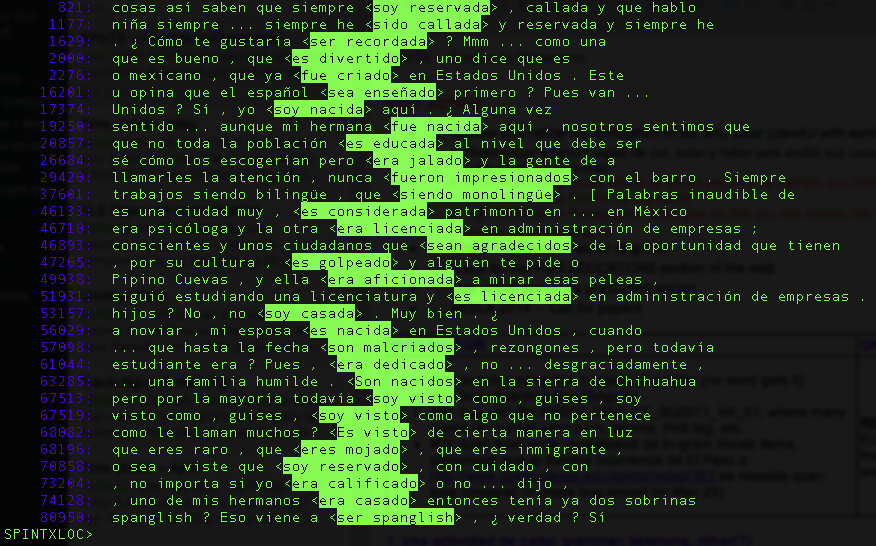
\includegraphics[scale=0.5]{Figs/InstancesOfSerPlusParticiple.png}

\caption{Ocurrencias de ser seguido de participio en Batch 1.}

\label{fig:InstancesOfSerPlusParticiple}

\end{figure}

\chapter{Funciones comunicativas}
\section{Expresar deseos con incertidumbre/en el futuro}
Esta sección contiene reglas que sirven para detectar estructuras lingüísticas generalmente utilizadas para expresar deseos que implican a uno mismo o a terceros. Esto hace, a menudo y según en qué construcciones, que sea necesario el subjuntivo. Así, por ejemplo, diremos ``me gustaría que te casaras conmigo'' para hacerle entender a nuestro interlocutor lo que deseamos que realice, pero en cambio diremos ``me gustaría casarme conmigo'' cuando queremos expresar que es nuestro deseo el que se realice. El primero usa subjuntivo y el segundo no.

\subsection{Expresar deseos con incertidumbre/en el futuro con agentes distintos en principal y subordinada}
\paragraph*{Rule}
\fbox{
\parbox{.9\linewidth}{\texttt{ADDRELATION (Func:Deseos:Ajenos) Verbo IF (0 VerbosExpresarDeseos) (1 Que) TO (*2 Verbo + Subjuntivo BARRIER GrupoNominal OR LimiteOracionSimple OR FiniteVerbForms);}}
}
\begin{itemize}
\item ETIQ: R:Func:Deseos:Ajenos
\item EJEM: (...) me sorprendió mi mamá porque no \emph{esperaba que me regalaran} nada (...)
\item DESC: Permite la presencia de clíticos entre el ``que'' y el subjuntivo que le sigue.
\end{itemize}

\paragraph*{Rule}
\fbox{
\parbox{.9\linewidth}{\texttt{ADDRELATION (Func:Deseos:Ajenos) Verbo IF (0 VerbosExpresarDeseos) (1 Adverbio OR MejorLiteral LINK 1 Que) TO (*3 Verbo + Subjuntivo BARRIER GrupoNominal OR LimiteOracionSimple OR FiniteVerbForms);}}
}
\begin{itemize}
\item ETIQ: R:Func:Deseos:Ajenos
\item EJEM: (...) me  \emph{gustaría mejor que te casaras} conmigo (...)
\item DESC: Permite la presencia de adverbios entre el verbo de la principal y el ``que''.
\end{itemize}

\paragraph*{Rule}
\fbox{
\parbox{.9\linewidth}{\texttt{ADDRELATION (Func:Deseos:Ajenos) Verbo IF (0 VerbosExpresarDeseos) (1 Que) (2 DetAllIncluded) (3 Sustantivo) (4 PronombresCliticosTODOS OR SeLiteral) TO (*5 Verbo + Subjuntivo BARRIER GrupoNominal OR LimiteOracionSimple OR FiniteVerbForms);}}
}
\begin{itemize}
\item ETIQ: R:Func:Deseos:Ajenos
\item EJEM: (...) \emph{espero que el español se vuelva} tal vez otro idioma oficial (...)
\item DESC: Permite la presencia de un sujeto entre el ``que'' y el subjuntivo.
\end{itemize}

\paragraph*{Rule}
\fbox{
\parbox{.9\linewidth}{\texttt{ADDRELATION (Func:Deseos:Ajenos) OjalaLiteral IF (0 OjalaLiteral) (1 Que) (2 DetAllIncluded) (3 Sustantivo) TO (*4 Verbo + Subjuntivo BARRIER GrupoNominal OR LimiteOracionSimple OR FiniteVerbForms);}}
}
\begin{itemize}
\item ETIQ: R:Func:Deseos:Ajenos
\item EJEM: Este ... \emph{ojalá que algún día cambie} , ¿ no ? Pero . ¿ Y tú opinas
\item DESC: Permite la presencia de un sintagma nominal sujeto entre el ``que'' y el subjuntivo.
\end{itemize}

\paragraph*{Rule}
\fbox{
\parbox{.9\linewidth}{\texttt{ADDRELATION (Func:Deseos:Ajenos) Verbo IF (0 VerbosExpresarDeseos) (1 DetAllIncluded) (2 Sustantivo OR Adj) (3 Que) (4 PronombresCliticosTODOS OR SeLiteral) TO (*5 Verbo + Subjuntivo BARRIER GrupoNominal OR LimiteOracionSimple OR FiniteVerbForms);}}
}
\begin{itemize}
\item ETIQ: R:Func:Deseos:Ajenos
\item EJEM: (...) no \emph{esperas tu niña que se comporte} así (...)
\item DESC: Permite un alteración sintáctica entre el sujeto de la subordinada y la posición del ``que''. Esto es algo inusual en la lengua escrita, pero dejamos la regla por si en el futuro permite detectar construcciones similares en la lengua oral.
\end{itemize}

\paragraph*{Rule}
\fbox{
\parbox{.9\linewidth}{\texttt{ADDRELATION (Func:Deseos:Ajenos) Sustantivo IF (0 NombresExpresarDeseos) (1 De OR Para) (2 Que) TO (*3 Verbo + Subjuntivo BARRIER LimiteOracionSimple OR FiniteVerbForms LINK T:SintagmaNominal-Y-O-Clitico);}}
}
\begin{itemize}
\item ETIQ: R:Func:Deseos:Ajenos
\item EJEM: (...) sin \emph{necesidad de que me tengan} que pagar.
\item DESC: Marca la ocurrencia de nombres como ``necesidad, petición'' seguidos de un ``para'' o un ``que'' y un verbo subjuntivo, y permite que aparezca un clítico o un sintagma nominal (Det N, Det Adj) entre el ``que'' y el verbo en subjuntivo.
\end{itemize}

REM: Esta regla utiliza el operador ``T:''. Esta ``T'' indica que los que sigue a los dos puntos (:) es un TEMPLATE definido más arriba, en la zona de definición de LIST y SET. Para más detalles véase la documentación vislcg3 y el grupo de debate (GoogleGroup).
\subsection{Expresar recomendaciones y sugerencias}
\paragraph*{Rule}
\fbox{
\parbox{.9\linewidth}{\texttt{ADDRELATION (Func:Sugerencias) Verbo IF (0 VerbosExpresarRecomendaciones) (1 Que) TO (*2 Verbo + Subjuntivo BARRIER LimiteOracionSimple OR FiniteVerbForms);}}
}
\begin{itemize}
\item ETIQ: Asigna la etiqueta R:Func:Sugerencias
\item EJEM: el médico les dice que él \emph{sugiere que apaguen} la máquina de  
\item DESC: NA.
\end{itemize}

\paragraph*{Rule}
\fbox{
\parbox{.9\linewidth}{\texttt{ADDRELATION (Func:Sugerencias) Verbo IF (0 VerbosExpresarRecomendaciones + 2aPers OR VerbosExpresarRecomendaciones + 3aPers) TO (1 Verbo + Infinitive);}}
}
\begin{itemize}
\item ETIQ: Asigna la etiqueta R:Func:Sugerencias
\item EJEM: mis amigos también fueron muy conscientes de que \emph{necesitaban hablar} un poquito más lento cuando estaban conmigo 
\item DESC: NA.
\end{itemize}

\paragraph*{Rule}
\fbox{
\parbox{.9\linewidth}{\texttt{ADDRELATION (Func:Sugerencias) Verbo IF (0 Ser + Verbo) (*1 AdjetivosUsadosEnRecomendaciones BARRIER LimiteOracionSimple OR FiniteVerbForms OR GrupoNominal) (2 Que) TO (*3 Verbo + Subjuntivo BARRIER LimiteOracionSimple OR FiniteVerbForms);}}
}
\begin{itemize}
\item ETIQ: Asigna la etiqueta R:Func:Sugerencias
\item EJEM: Usted cree que va a \emph{ser importante} que le enseñen a sus nietos los dos idiomas 
\item DESC: NA.
\end{itemize}

\paragraph*{Rule}
\fbox{
\parbox{.9\linewidth}{\texttt{ADDRELATION (Func:Sugerencias) Verbo IF (NOT -1 Que LINK -1 VerbosOpinionLema + 2aPers) (0 Ser + Verbo) (*1 AdjetivosUsadosEnRecomendaciones BARRIER LimiteOracionSimple OR FiniteVerbForms OR GrupoNominal) TO (*2 Verbo + Infinitive BARRIER LimiteOracionSimple OR FiniteVerbForms LINK NOT 0 Ser);}}
}
\begin{itemize}
\item ETIQ: Asigna la etiqueta R:Func:Sugerencias
\item EJEM: Ahorita mucha gente lo sabe hablar y \emph{es importante saber} comunicarte con otra gente
\item DESC: NA.
\end{itemize}

REM: Existen otros usos de necesitar, más parecidos a requerir como por ejemple (1)  [...] sería muy , muy interesante , pero por ejemplo para ese trabajo ``necesitas ser'' ciudadano , así que es ... es muy importante o (2) [...] yo estoy más que dispuesta a trabajar con usted nada más ``necesito estar'' en casa cuando AISD no tiene clases. Ambas oraciones muestran un uso que no está claro que sea un consejo o una recomendación, especialmente la primera. Ambas son necesidades, requerimientos externos o personales.
\section{Expresar objetivos y finalidades con ``para''}
\paragraph*{Rule}
\fbox{
\parbox{.9\linewidth}{\texttt{ADDRELATION (Func:Finalidades) Prep IF (0 Para) (1 Verbo + Infinitive) TO (*2 Que BARRIER LimiteOracionSimple OR FiniteVerbForms LINK 1 Verbo + Subjuntivo);}}
}
\begin{itemize}
\item ETIQ: R:Func:Finalidades
\item EJEM: (...) Yo crecí pensando que para orar o \emph{para pedirle a Dios que hiciera algo} (...)
\item DESC: NA.
\end{itemize}

\subsection{Estilo indirecto}
\subsection{Expresando opiniones}
\subsection{Dar opiniones}
\paragraph*{Rule}
\fbox{
\parbox{.9\linewidth}{\texttt{ADDRELATION (Func:Opiniones:Dar) DetPosSingTODOS IF (0 DetPosSingTODOS) (1 PuntoLema) (2 De) TO (3 VistaLiteral);}}
}
\paragraph*{Rule}
\fbox{
\parbox{.9\linewidth}{\texttt{ADDRELATION (Func:Opiniones:Dar) (NEG) IF (0 No) (1 Ser + Verbo) (2 TanLema) (3 Adj) TO (**5 VerbosOpinionLema + Verbo + PasadoIndicativo BARRIER FiniteVerbForms OR LimiteOracionSimpleMenosComo LINK -1 ComoLema);}}
}
\paragraph*{Rule}
\fbox{
\parbox{.9\linewidth}{\texttt{ADDRELATION (Func:Opiniones:Dar) Verbo IF (NOT -1 QueConAcento) (0 Ser + Verbo) (*1 AdjetivosExpresarOpiniones BARRIER LimiteOracionSimple OR FiniteVerbForms OR GrupoNominal) TO (*2 Verbo + Infinitive BARRIER LimiteOracionSimple OR FiniteVerbForms LINK NOT 0 Ser);}}
}
\paragraph*{Rule}
\fbox{
\parbox{.9\linewidth}{\texttt{ADDRELATION (Func:Opiniones:Dar) (CQUE) IF (0 Que) (1 VerbosOpinionLema) TO (2 Que);}}
}
\begin{itemize}
\item ETIQ: R:Func:Opinion:Dar
\item EJEM: (...) está mal, en mi ... en \emph{mi punto de vista}, porque se va perdiendo (...)
\item DESC: NA.
\end{itemize}

\subsection{Pedir opiniones}
\paragraph*{Rule}
\fbox{
\parbox{.9\linewidth}{\texttt{ADDRELATION (Func:Opiniones:Pedir) (PPX) IF (0 TuLiteral) (1 VerbosOpinionLema + Verbo + 2aPers) TO (2 Que);}}
}
\paragraph*{Rule}
\fbox{
\parbox{.9\linewidth}{\texttt{ADDRELATION (Func:Opiniones:Pedir) Adverbio IF (0 ComoAcento OR ("<entonces>"i)) (1 VerbosOpinionLema + Verbo + 2aPers) TO (2 Que);}}
}
\paragraph*{Rule}
\fbox{
\parbox{.9\linewidth}{\texttt{ADDRELATION (Func:Opiniones:Pedir) (INT) IF (0 QueConAcento OR CualConAcento) (1 VerbosOpinionLema + Verbo + 2aPers) TO (2 Que);}}
}
\paragraph*{Rule}
\fbox{
\parbox{.9\linewidth}{\texttt{ADDRELATION (Func:Opiniones:Pedir) Puntuacion IF (0 InterroganteInicial) (1 VerbosOpinionLema + Verbo + 2aPers) TO (2 Que);}}
}
\paragraph*{Rule}
\fbox{
\parbox{.9\linewidth}{\texttt{ADDRELATION (Func:Opiniones:Pedir) (CC) IF (0 YLiteral OR ConjLetraO) (1 VerbosOpinionLema + Verbo + 2aPers) TO (2 Que);}}
}
\paragraph*{Rule}
\fbox{
\parbox{.9\linewidth}{\texttt{ADDRELATION (Func:Opiniones:Pedir) (NEG) IF (0 No) (1 VerbosOpinionLema + Verbo + 2aPers) TO (2 Que);}}
}
\subsection{Expresando sorpresa}
\paragraph*{Rule}
\fbox{
\parbox{.9\linewidth}{\texttt{ADDRELATION (Func:Sorpresa) No IF (0 No) (1 PoderLema + Verbo) (2 CreerLema) TO (3 Que);}}
}
\paragraph*{Rule}
\fbox{
\parbox{.9\linewidth}{\texttt{ADDRELATION (Func:Sorpresa) No IF (0 No) (1 LoLiteral) (2 PoderLema + Verbo) TO (3 CreerLema);}}
}
\begin{itemize}
\item ETIQ: R:Func:Sorpresa
\item EJEM: (...) \emph{no puedo creer que}, porque se va perdiendo (...)
\item DESC: NA.
\end{itemize}

\section{Expresar opiniones, dudas}
\section{Expresar necesidades}
\paragraph*{Rule}
\fbox{
\parbox{.9\linewidth}{\texttt{ADDRELATION (Func:Necesidades) Verbo (0 NecesitarLema) TO (**1 SustantivosQueDenotanNecesidades + Nombre BARRIER LimiteOracionSimple OR FiniteVerbForms);}}
}
\begin{itemize}
\item ETIQ: R:Func:Necesidades
\item EJEM: si \emph{necesitan ayuda} en algo
\item DESC: NA
\end{itemize}

\paragraph*{Rule}
\fbox{
\parbox{.9\linewidth}{\texttt{ADDRELATION (Func:Necesidades) LoLiteral (0 LoLiteral) (NOT 0 YaAnotadoComoNecesidad) (1 Que) TO (2 NecesitarLema + Verbo); }}
}
\begin{itemize}
\item ETIQ: R:Func:Necesidades
\item EJEM: \emph{lo que necesitaba} yo para
\item DESC: NA
\end{itemize}

\paragraph*{Rule}
\fbox{
\parbox{.9\linewidth}{\texttt{ADDRELATION (Func:Necesidades) TuLiteral (0 TuLiteral) (NOT 0 YaAnotadoComoNecesidad) (1 QueConAcento) TO (2 NecesitarLema + Verbo); }}
}
\begin{itemize}
\item ETIQ: R:Func:Necesidades
\item EJEM: \emph{tú qué necesitas}, muchachita
\item DESC: NA
\end{itemize}

\paragraph*{Rule}
\fbox{
\parbox{.9\linewidth}{\texttt{ADDRELATION (Func:Necesidades) Verbo (0 NecesitarLema) (NOT 0 YaAnotadoComoNecesidad) (1 APrep) TO (*2 DetAllIncluded OR NombrePropio OR Dios BARRIER LimiteOracionSimple OR FiniteVerbForms LINK NOT 0 Articulo);  }}
}
\begin{itemize}
\item ETIQ: R:Func:Necesidades
\item EJEM: \emph{necesito a Jill} en mi vida.
\item DESC: NA
\end{itemize}

\paragraph*{Rule}
\fbox{
\parbox{.9\linewidth}{\texttt{ADDRELATION (Func:Necesidades) Verbo (0 NecesitarLema) (NOT 0 YaAnotadoComoNecesidad) (1 APrep) TO (*2 DetAllIncluded BARRIER LimiteOracionSimple OR FiniteVerbForms OR Prep LINK 1 Sustantivo);}}
}
\begin{itemize}
\item ETIQ: R:Func:Necesidades
\item EJEM: \emph{necesito a un profesor} de inglés.
\item DESC: NA
\end{itemize}

\paragraph*{Rule}
\fbox{
\parbox{.9\linewidth}{\texttt{ADDRELATION (Func:Necesidades) Verbo (0 NecesitarLema) (NOT 0 YaAnotadoComoNecesidad) TO (*1 DetAllIncluded BARRIER LimiteOracionSimple OR FiniteVerbForms OR Prep LINK 1 Sustantivo); }}
}
\begin{itemize}
\item ETIQ: R:Func:Necesidades
\item EJEM: ellos \emph{necesitan las persona} a su lado y
\item EJEM: \emph{necesitas resolver tus problemas}.
\item DESC: NA
\end{itemize}

\paragraph*{Rule}
\fbox{
\parbox{.9\linewidth}{\texttt{ADDRELATION (Func:Necesidades) Verbo (0 Ser) TO (**1 NecesarioLema BARRIER LimiteOracionSimple OR FiniteVerbForms OR Prep); }}
}
\begin{itemize}
\item ETIQ: R:Func:Necesidades
\item EJEM: (no) \emph{es algo muy necesario}
\item DESC: NA
\end{itemize}

\paragraph*{Rule}
\fbox{
\parbox{.9\linewidth}{\texttt{ADDRELATION (Func:Necesidades) (Determiner) (0 DetAllIncluded) (1 Sustantivo) TO (2 NecesarioLema);}}
}
\begin{itemize}
\item ETIQ: R:Func:Necesidades
\item EJEM: \emph{los materiales necesarios}
\item DESC: NA
\end{itemize}

\paragraph*{Rule}
\fbox{
\parbox{.9\linewidth}{\texttt{ADDRELATION (Func:Agradecer) (Determiner) (0 MuchoLema) (1 Gracia + PL) TO (2 Por);}}
}
\begin{itemize}
\item ETIQ: R:Func:Agradecer
\item EJEM: \emph{muchas gracias por}
\item DESC: NA
\end{itemize}

\paragraph*{Rule}
\fbox{
\parbox{.9\linewidth}{\texttt{ADDRELATION (Func:Agradecer) (Determiner) (0 MuchoLema) (1 Gracia + PL) (2 PuntuacionComa) TO (3 NombrePropio);}}
}
\begin{itemize}
\item ETIQ: R:Func:Agradecer
\item EJEM: \emph{muchas gracias, Sabrina}
\item DESC: NA
\end{itemize}

\paragraph*{Rule}
\fbox{
\parbox{.9\linewidth}{\texttt{ADDRELATION (Func:Agradecer) Nombre (0 Gracia + PL) (1 APrep) TO (2 NombrePropio OR PronPersFuerte OR Dios);}}
}
\begin{itemize}
\item ETIQ: R:Func:Agradecer
\item EJEM: \emph{gracias a Dios}, \emph{gracias a él}
\item DESC: NA
\end{itemize}

\paragraph*{Rule}
\fbox{
\parbox{.9\linewidth}{\texttt{ADDRELATION (Func:Agradecer) Nombre (0 Gracia + PL) TO (1 APrep LINK T:SintagmaNominalHaciaLaIzda);}}
}
\begin{itemize}
\item ETIQ: R:Func:Agradecer
\item EJEM: \emph{gracias a la tecnología}
\item DESC: NA
\end{itemize}

\paragraph*{Rule}
\fbox{
\parbox{.9\linewidth}{\texttt{ADDRELATION (Func:Agradecer) Verbo (0 DarLema + Verbo) TO (**1 Gracia + PL BARRIER LimiteOracionSimple OR FiniteVerbForms OR Prep);}}
}
\begin{itemize}
\item ETIQ: R:Func:Agradecer
\item EJEM: \emph{damos las gracias}, \emph{darle gracias}
\item DESC: NA
\end{itemize}

\paragraph*{Rule}
\fbox{
\parbox{.9\linewidth}{\texttt{ADDRELATION (Func:Agradecer) LeLema (0 LeLema) (1 AgradecerLema + Verbo) TO (1 MuchoLema);}}
}
\begin{itemize}
\item ETIQ: R:Func:Agradecer
\item EJEM: \emph{le agradezco mucho} a ella
\item DESC: NA
\end{itemize}

\paragraph*{Rule}
\fbox{
\parbox{.9\linewidth}{\texttt{ADDRELATION (Func:Agradecer) PronPersFuerte (0 PronPersFuerte) (1 AgradecerLema + Verbo) TO (2 ArtPronDemo);}}
}
\paragraph*{Rule}
\fbox{
\parbox{.9\linewidth}{\texttt{ADDRELATION (Func:Agradecer) Verbo (0 AgradecerLema + Gerundio) TO (**2 Que BARRIER LimiteOracionSimple OR FiniteVerbForms OR Prep LINK -1 LoLiteral);}}
}
\begin{itemize}
\item ETIQ: R:Func:Agradecer
\item EJEM: \emph{yo agradezco eso}
\item EJEM: \emph{agradeciendo lo que tienes}
\item DESC: NA
\end{itemize}

\section{Expresar ayuda}
\subsection{Pedir ayuda}
\paragraph*{Rule}
\fbox{
\parbox{.9\linewidth}{\texttt{ADDRELATION (Func:Ayuda:Pedir) PronombreDeObjetoPrimeraPersona (0 PronombreDeObjetoPrimeraPersona) (1 PoderLema + Verbo + 2aPers OR PoderLema + Verbo + 3aPers) TO (**2 AyudarLema + Verbo BARRIER LimiteOracionSimple OR FiniteVerbForms);}}
}
\begin{itemize}
\item ETIQ: R:Func:Ayuda:Pedir
\item EJEM: \emph{me puedes ayudar} a hacer las tortitas
\item DESC: NA
\end{itemize}

\paragraph*{Rule}
\fbox{
\parbox{.9\linewidth}{\texttt{ADDRELATION (Func:Ayuda:Pedir) Verbo (NOT -1 PronombreDeObjetoPrimeraPersona) (0 PoderLema + Verbo + 2aPers OR PoderLema + Verbo + 3aPers) TO (**1 AyudarLema + Verbo BARRIER LimiteOracionSimple OR FiniteVerbForms);}}
}
\begin{itemize}
\item ETIQ: R:Func:Ayuda:Ofrecer
\item EJEM: \emph{Puedes empezar a ayudarnos} a (...)
\item DESC: NA
\end{itemize}

\paragraph*{Rule}
\fbox{
\parbox{.9\linewidth}{\texttt{ADDRELATION (Func:Ayuda:Pedir) Verbo (0 LemasQueSeAsemejanANecesitar + Verbo) TO (**1 AyudarLema + Verbo BARRIER LimiteOracionSimple OR FiniteVerbForms);}}
}
\begin{itemize}
\item ETIQ: R:Func:Ayuda:Ofrecer
\item EJEM: si uno \emph{necesita algo ellos mismos nos ayudan}
\item DESC: NA
\end{itemize}

\subsection{Ofrecer ayuda}
\paragraph*{Rule}
\fbox{
\parbox{.9\linewidth}{\texttt{ADDRELATION (Func:Ayuda:Ofrecer) Puntuacion (0 InterroganteInicial) TO (**3 InterroganteFinal BARRIER LimiteOracionSimple OR FiniteVerbForms LINK *-1 AyudaLema + Nombre LINK -1 LemasQueSeAsemejanANecesitar + Verbo);}}
}
\begin{itemize}
\item ETIQ: R:Func:Ayuda:Ofrecer
\item EJEM: \emph{¿necesitas ayuda?}
\item DESC: NA
\end{itemize}

\paragraph*{Rule}
\fbox{
\parbox{.9\linewidth}{\texttt{ADDRELATION (Func:Ayuda:Ofrecer) Verbo (0 Haber + FiniteVerbForms) (1 LemasQueSeAsemejanANecesitar + Part) TO (**2 AyudaLema + Nombre BARRIER LimiteOracionSimple OR FiniteVerbForms);}}
}
\begin{itemize}
\item ETIQ: R:Func:Ayuda:Ofrecer
\item EJEM: \emph{ha requerido la ayuda de}
\item DESC: NA
\end{itemize}

\section{Referir palabras ya dichas}
\subsection{Referir palabras propias}
\paragraph*{Rule}
\fbox{
\parbox{.9\linewidth}{\texttt{ADDRELATION (Func:Referir) PronombresCliticosTODOS (0 PronombresCliticosTODOS) (1 VerbiDicendi + PretPerfSimple + 1aPers) To (2 Que);}}
}
\paragraph*{Rule}
\fbox{
\parbox{.9\linewidth}{\texttt{ADDRELATION (Func:Referir) PronombresCliticosTODOS (0 PronombresCliticosTODOS) (1 VerbiDicendiConSi + PretPerfSimple + 1aPers) To (2 SiLema);}}
}
\paragraph*{Rule}
\fbox{
\parbox{.9\linewidth}{\texttt{ADDRELATION (Func:Referir) PronombresCliticosTODOS (0 PronombresCliticosTODOS) (1 VerbiDicendiConSi + PretPerfSimple + 1aPers) To (*2 SiLema BARRIER LimiteOracionSimpleMenosQue OR FiniteVerbForms LINK -1 Que);}}
}
\paragraph*{Rule}
\fbox{
\parbox{.9\linewidth}{\texttt{ADDRELATION (Func:Referir) Verbo (NOT -1 PronombresCliticosTODOS) (0 VerbiDicendi + PretPerfSimple + 1aPers) To (1 Que);}}
}
\paragraph*{Rule}
\fbox{
\parbox{.9\linewidth}{\texttt{ADDRELATION (Func:Referir) Verbo (NOT -1 PronombresCliticosTODOS) (0 VerbiDicendiConSi + PretPerfSimple + 1aPers) To (1 SiLema);}}
}
\begin{itemize}
\item ETIQ: R:Func:Referir
\item EJEM: \emph{le dije que si}
\item EJEM: con la maestra \emph{le pedí que si} (...)
\item DESC: NA
\end{itemize}

\subsection{Referir palabras de otros}
\paragraph*{Rule}
\fbox{
\parbox{.9\linewidth}{\texttt{ADDRELATION (Func:Referir) PronombresCliticosTODOS (0 PronombresCliticosTODOS) (1 VerbiDicendi + PretPerfSimple) (NOT 1 1aPers) To (2 Que);}}
}
\paragraph*{Rule}
\fbox{
\parbox{.9\linewidth}{\texttt{ADDRELATION (Func:Referir) PronombresCliticosTODOS (0 PronombresCliticosTODOS) (1 VerbiDicendiConSi + PretPerfSimple) (NOT 1 1aPers) To (2 SiLema);}}
}
\paragraph*{Rule}
\fbox{
\parbox{.9\linewidth}{\texttt{ADDRELATION (Func:Referir) PronombresCliticosTODOS (0 PronombresCliticosTODOS) (1 VerbiDicendiConSi + PretPerfSimple) (NOT 1 1aPers) To (*2 SiLema BARRIER LimiteOracionSimpleMenosQue OR FiniteVerbForms LINK -1 Que);}}
}
\paragraph*{Rule}
\fbox{
\parbox{.9\linewidth}{\texttt{ADDRELATION (Func:Referir) Verbo (NOT -1 PronombresCliticosTODOS) (0 VerbiDicendi + PretPerfSimple) (NOT 1 1aPers) To (1 Que);}}
}
\paragraph*{Rule}
\fbox{
\parbox{.9\linewidth}{\texttt{ADDRELATION (Func:Referir) Verbo (NOT -1 PronombresCliticosTODOS) (0 VerbiDicendiConSi + PretPerfSimple) (NOT 1 1aPers) To (1 SiLema);}}
}
\begin{itemize}
\item ETIQ: R:Func:Referir
\item EJEM: \emph{le preguntó que si} quería (...)
\item EJEM: ¿alguna vez \emph{les dijo que} no mezclaran (...)
\item DESC: NA
\end{itemize}

\section{Describir personas}
\section{Describir el caràcter de las personas}
\paragraph*{Rule}
\fbox{
\parbox{.9\linewidth}{\texttt{ADDRELATION (Func:DescribirPersonas:FormaDeSer) Verbo (0 VerboEstar OR Ser) TO (*1 AdvIntensificadorAdjetivos BARRIER LimiteOracionSimple OR Verbo OR NombresNoDePersonalidad OR Prep LINK 1 AdjetivosParaDescribirCaracterPersonas OR VerbosQueEnParticipioPuedenDescribirCaracteres + Part LINK NOT 0 MaloLiteral LINK NOT 1 ReferenciaALugar OR PronDemoNeutro);}}
}
\begin{itemize}
\item ETIQ: R:Func:DescribirPersonas:FormaDeSer
\item EJEM: \emph{era la más tímida}
\item DESC: NA
\end{itemize}

\paragraph*{Rule}
\fbox{
\parbox{.9\linewidth}{\texttt{ADDRELATION (Func:DescribirPersonas:FormaDeSer) Verbo (0 VerboEstar OR Ser) (NOT -1 QueConAcento) TO (1 AdjetivosParaDescribirCaracterPersonas OR VerbosQueEnParticipioPuedenDescribirCaracteres + Part LINK NOT 0 MaloLiteral LINK NOT 1 ReferenciaALugar OR PronDemoNeutro);}}
}
\begin{itemize}
\item ETIQ: R:Func:DescribirPersonas:FormaDeSer
\item EJEM: yo \emph{he sido callada} y reservada
\item EJEM: \emph{Era trabajadora} y reservada
\item DESC: NA
\end{itemize}

\paragraph*{Rule}
\fbox{
\parbox{.9\linewidth}{\texttt{ADDRELATION (Func:DescribirPersonas:FormaDeSer) AdjOrPart (0 AdjetivosParaDescribirCaracterPersonas OR VerbosQueEnParticipioPuedenDescribirCaracteres + Part) (1 PuntuacionComa OR YLiteral) TO (2 AdjetivosParaDescribirCaracterPersonas OR VerbosQueEnParticipioPuedenDescribirCaracteres + Part);}}
}
\begin{itemize}
\item ETIQ: R:Func:DescribirPersonas:FormaDeSer
\item EJEM: en cierto punto \emph{callada, amigable} (...)
\item DESC: NA
\end{itemize}

\paragraph*{Rule}
\fbox{
\parbox{.9\linewidth}{\texttt{ADDRELATION (Func:DescribirPersonas:FormaDeSer) DetAllIncluded (0 DetAllIncluded) (NOT 0 LoLiteral) TO (1 AdvIntensificadorAdjetivos LINK 1 AdjetivosParaDescribirCaracterPersonas OR VerbosQueEnParticipioPuedenDescribirCaracteres + Part);}}
}
\begin{itemize}
\item ETIQ: R:Func:DescribirPersonas:FormaDeSer
\item EJEM: \emph{la más tímida}
\item DESC: No precedido de ser o estar.
\end{itemize}

\section{Expresar objetivos (con para que)}
OBSERVACIÓN: Oración sacada del corpus. 45388:  que viene a vivir a ? . ¿ Qué le <recomendaría> a un hispano que viene a vivir a o a (...) . Esta frase anterior no es la misma construcción (que la de los deseos con sjubjuntivo) porque el que ``viene a vivir'' es una adjetival de hispano, no una subordinada de recomendar.

OBSERVACIÓN:  Oración sacada del corpus. 45410:  Estados Unidos ? , más como yo . Yo le <recomendaría> , en cuanto al idioma , trate de aprenderlo lo (...) Esta oración refleja la omisión del que (oral o literario, algo recargado). Este tipo de estructuras requerirían un análisis lingüístico más sofisticado, seguramente -- sintáctico, análisis de incisos, etc.

\section{Expresar deseos y recomendaciones (implicando a uno mismo)}
\chapter{Pragmática}
\section{Marcadores discursivos}
Véase \url{http://www.cs.famaf.unc.edu.ar/~laura/shallowdisc4summ/index.html}.

\subsection{Marcadores discursivos indicadores de revisión}
\paragraph*{Rule}
\fbox{
\parbox{.9\linewidth}{\texttt{ADD (@Prag:MarcadoresDisc:Revision) MarcDiscRevision;}}
}
\begin{itemize}
\item ETIQ: @:Prag:MarcadoresDisc:Revision
\item EJEM: \emph{aunque}, \emph{excepto} o \emph{pero}
\item DESC: [Espacio para describir con palabras lo que hace la regla.]
\end{itemize}

\paragraph*{Rule}
\fbox{
\parbox{.9\linewidth}{\texttt{ADDRELATION (Prag:MarcadoresDisc:Revision) Sin TO (1 Embargo);}}
}
\begin{itemize}
\item ETIQ: R:Prag:MarcadoresDisc:Revision (relación entre el primer i el último elemento de la locución)
\item EJEM: \emph{sin embargo}
\item DESC: [Espacio para describir con palabras lo que hace la regla.]
\end{itemize}

\paragraph*{Rule}
\fbox{
\parbox{.9\linewidth}{\texttt{ADDRELATION (Prag:MarcadoresDisc:Revision) De TO (1 Hecho);}}
}
\begin{itemize}
\item ETIQ: R:Prag:MarcadoresDisc:Revision (relación entre el primer i el último elemento de la locución)
\item EJEM: \emph{de hecho}
\item DESC: [Espacio para describir con palabras lo que hace la regla.]
\end{itemize}

\paragraph*{Rule}
\fbox{
\parbox{.9\linewidth}{\texttt{ADDRELATION (Prag:MarcadoresDisc:Revision) En TO (1 Realidad);}}
}
\begin{itemize}
\item ETIQ: R:Prag:MarcadoresDisc:Revision (relación entre el primer i el último elemento de la locución)
\item EJEM: \emph{en realidad}
\item DESC: [Espacio para describir con palabras lo que hace la regla.]
\end{itemize}

\paragraph*{Rule}
\fbox{
\parbox{.9\linewidth}{\texttt{ADDRELATION (Prag:MarcadoresDisc:Revision) APrep (1 Pesar) TO (2 De);}}
}
\begin{itemize}
\item ETIQ: R:Prag:MarcadoresDisc:Revision (relación entre el primer i el último elemento de la locución)
\item EJEM: \emph{a pesar de}
\item DESC: [Espacio para describir con palabras lo que hace la regla.]
\end{itemize}

\paragraph*{Rule}
\fbox{
\parbox{.9\linewidth}{\texttt{ADDRELATION (Prag:MarcadoresDisc:Revision) De (1 Todos) TO (2 Modos);}}
}
\begin{itemize}
\item ETIQ: R:Prag:MarcadoresDisc:Revision (relación entre el primer i el último elemento de la locución)
\item EJEM: \emph{de todos modos}
\item DESC: [Espacio para describir con palabras lo que hace la regla.]
\end{itemize}

\paragraph*{Rule}
\fbox{
\parbox{.9\linewidth}{\texttt{ADDRELATION (Prag:MarcadoresDisc:Revision) Es (1 Cierto) TO (2 Que);}}
}
\begin{itemize}
\item ETIQ: R:Prag:MarcadoresDisc:Revision (relación entre el primer i el último elemento de la locución)
\item EJEM: \emph{s cierto que}
\item DESC: [Espacio para describir con palabras lo que hace la regla.]
\end{itemize}

\subsection{Marcadores discursivos indicadores de causa}
\paragraph*{Rule}
\fbox{
\parbox{.9\linewidth}{\texttt{ADD (@Prag:MarcadoresDisc:Causa) Porque;}}
}
\begin{itemize}
\item ETIQ: @Prag:MarcadoresDisc:Causa
\item DESC: [Espacio para describir con palabras lo que hace la regla.]
\end{itemize}

\paragraph*{Rule}
\fbox{
\parbox{.9\linewidth}{\texttt{ADDRELATION (Prag:MarcadoresDisc:Causa) Prep IF (0 Por) (1 LoLiteral) TO (2 Tanto);}}
}
\paragraph*{Rule}
\fbox{
\parbox{.9\linewidth}{\texttt{ADDRELATION (Prag:MarcadoresDisc:Causa) Prep IF (0 Por) TO (2 Tanto OR FormasDePalabrasEnLocucionesCausalesConPor);}}
}
\begin{itemize}
\item ETIQ: Asigna @Prag:MarcadoresDisc:Causa.
\item EJEM: \emph{por lo tanto}
\item EJEM: \emph{por eso}
\item DESC: Requiere \emph{por} seguida por LO y TANTO
\end{itemize}

\paragraph*{Rule}
\fbox{
\parbox{.9\linewidth}{\texttt{ADDRELATION (Prag:MarcadoresDisc:Causa) Debido TO (1 APrep);}}
}
\begin{itemize}
\item ETIQ: R:Prag:MarcadoresDisc:Causa (relación entre el primer i el último elemento de la locución)
\item DESC: [Espacio para describir con palabras lo que hace la regla.]
\end{itemize}

\paragraph*{Rule}
\fbox{
\parbox{.9\linewidth}{\texttt{ADDRELATION (Prag:MarcadoresDisc:Causa) Nombre (0 Gracia + PL) TO (1 APrep);}}
}
\begin{itemize}
\item ETIQ: R:Prag:MarcadoresDisc:Causa (relación entre el primer i el último elemento de la locución)
\item DESC: [Espacio para describir con palabras lo que hace la regla.]
\end{itemize}

\subsection{Marcadores discursivos indicadores de igualdad}
\paragraph*{Rule}
\fbox{
\parbox{.9\linewidth}{\texttt{ADD (@Prag:MarcadoresDisc:Igualdad) Adverbio IF (0 Ademas) (NOT 1 De);}}
}
\paragraph*{Rule}
\fbox{
\parbox{.9\linewidth}{\texttt{ADD (@Prag:MarcadoresDisc:Igualdad) Adverbio IF (0 Tambien);}}
}
OBSERVACIÓN: No añado \emph{precisamente} porque es ambiguo entre su lectura literal (preciso, justo, cierto) como modificador verbal y su lectura como marcador discursivo. Para anotarlo con fiabilidad habría que tener en cuenta su posición respecto al principio de la oración y el verbo principal. Ejemplos: \emph{sí muchas pero no sé precisamente cuál cuál sería una}, \emph{allí vivimos como un año y precisamente yo me tomé me tomaron fotos en un un estudio de fotografía}

\begin{itemize}
\item ETIQ: @:Prag:MarcadoresDisc:Igualdad
\item EJEM: \emph{además}, \emph{también}
\item DESC: Requiere \emph{además} o \emph{también} no seguido de DE
\end{itemize}

\paragraph*{Rule}
\fbox{
\parbox{.9\linewidth}{\texttt{ADDRELATION (Prag:MarcadoresDisc:Igualdad) Prep IF (0 Por) TO (1 Ejemplo);}}
}
\begin{itemize}
\item ETIQ: R:Prag:MarcadoresDisc:Igualdad (relación entre el primer i el último elemento de la locución)
\item EJEM: \emph{por ejemplo}
\item DESC: Requiere \emph{por} seguida por alguna palabra en la lista de palabras predefinidas \emph{LemasDePalabrasEnLocucionesConPor}
\end{itemize}

\paragraph*{Rule}
\fbox{
\parbox{.9\linewidth}{\texttt{ADDRELATION (Prag:MarcadoresDisc:Igualdad) ConjLetraO TO (1 Sea);}}
}
\begin{itemize}
\item ETIQ: R:Prag:MarcadoresDisc:Igualdad
\item EJEM: \emph{o sea}
\item DESC: NA.
\end{itemize}

\paragraph*{Rule}
\fbox{
\parbox{.9\linewidth}{\texttt{ADDRELATION (Prag:MarcadoresDisc:Igualdad) No TO (1 SoloAcento);}}
}
\begin{itemize}
\item ETIQ: R:Prag:MarcadoresDisc:Igualdad
\item EJEM: porque uno \emph{no sólo} puede ayudar en el aspecto de inglés pero en el aspecto del español también
\item DESC: NA.
\end{itemize}

\paragraph*{Rule}
\fbox{
\parbox{.9\linewidth}{\texttt{ADD (@Prag:MarcadoresDisc:Probabilidad) Adverbio IF (0 QuizasConOSinEse);}}
}
\begin{itemize}
\item ETIQ: R:Prag:MarcadoresDisc:Probabilidad
\item EJEM: (...) lo que sí me gustaría es que \emph{quizás} no tuvieran un acento muy marcado (...)
\item DESC: NA.
\end{itemize}

\paragraph*{Rule}
\fbox{
\parbox{.9\linewidth}{\texttt{ADDRELATION (Prag:MarcadoresDisc:Probabilidad) Tal TO (1 Vez);}}
}
\begin{itemize}
\item ETIQ: R:Prag:MarcadoresDisc:Probabilidad
\item EJEM: noto que \emph{tal vez} sus hijos hablan el spanglish más unos más que otros
\item DESC: NA.
\end{itemize}

\paragraph*{Rule}
\fbox{
\parbox{.9\linewidth}{\texttt{ADDRELATION (Prag:MarcadoresDisc:Probabilidad) APrep (1 LoLiteral) TO (2 MejorLiteral);}}
}
\begin{itemize}
\item ETIQ: R:Prag:MarcadoresDisc:Probabilidad
\item EJEM: Pero, \emph{a lo mejor} era no más porque estaba chiquita (...)
\item DESC: NA.
\end{itemize}

\subsection{Elementos discursivos usadors para ganar tiempo}
\paragraph*{Rule}
\fbox{
\parbox{.9\linewidth}{\texttt{ADD (@Prag:RecuDiscurso:GanarTiempo) ArtPronDemo IF (NOT -1 Prep) (0 EsteLiteral) (NOT 1 Nombre);}}
}
\begin{itemize}
\item ETIQ: @Prag:ElementosDiscurso:GanarTiempo
\item EJEM: \emph{Este} en mi niñez era un poco más soñadora mucho más soñadora de hecho (...)
\item DESC: Anota ocurrencies de ESTE que no vayan precedidas de una preposición ni seguidas de un sustantivo.
\end{itemize}

\chapter{Estructuras características del habla en hablantes de herencia}
\section{Estructuras derivadas del contacto entre lenguas}
\subsection{Expresiones con cambio de código}
Incluímos aquí expresiones que mezclan palabras en ambas lenguas, en este caso el español y el inglés. En la bibliografía especializada se utiliza el término inglés ``code switching''.

\paragraph*{Rule}
\fbox{
\parbox{.9\linewidth}{\texttt{ADDRELATION (Herit:Contacto:Mixtas) Verbo IF (0 ListaVerbosCorpusParaContactoMixtos) TO (*1 PalabraEnIngles BARRIER PalabraEnEspanol);}}
}
\begin{itemize}
\item ETIQ: R:Herit:Contacto:Mixtas
\item EJEM: \emph{hacer request}, \emph{comer turkey}
\item DESC: Anota secuencias de un verbo seguid de una o más palabras en inglés. Por ahora lo limitamos a ser, hacer, decir y comer porque TreeTagger anota como verbo algunas palabras que no lo son y no queremos generar ruido para los usuarios.
\end{itemize}

\paragraph*{Rule}
\fbox{
\parbox{.9\linewidth}{\texttt{ADDRELATION (Herit:Contacto:Mixtas) (Determiner) IF (0 DetAllIncluded) TO (**1 PalabraEnIngles BARRIER PalabraEnEspanol);}}
}
\section{Usos de inidicativo dónde se esperaría subjuntivo (en español estándard)}
OBSERVACIÓN: Sección en proceso de implementación.

\chapter{Vocabulario multipalabra}
\section{Nombres propios}
\subsection{Nombres de localizaciones geográficas}
\paragraph*{Rule}
\fbox{
\parbox{.9\linewidth}{\texttt{ADDRELATION (Vocab:Entities:Geo) Articulo IF  (0 ("<El>")) TO (1 ("<Paso>"));}}
}
\paragraph*{Rule}
\fbox{
\parbox{.9\linewidth}{\texttt{ADDRELATION (Vocab:Entities:Geo) Nombre IF  (0 ("<Estados>")) TO (1 ("<Unidos>"));}}
}
\paragraph*{Rule}
\fbox{
\parbox{.9\linewidth}{\texttt{ADDRELATION (Vocab:Entities:Geo) Nombre IF  (0 ("<Ciudad>")) TO (1 ("<Juárez>"));}}
}
\paragraph*{Rule}
\fbox{
\parbox{.9\linewidth}{\texttt{ADDRELATION (Vocab:Entities:Geo) Nombre IF  (0 ("<Rancho>")) TO (1 ("<Viejo>"));}}
}
\paragraph*{Rule}
\fbox{
\parbox{.9\linewidth}{\texttt{ADDRELATION (Vocab:Entities:Geo) Adj IF  (0 ("<Buenos>")) TO (1 ("<Aires>"));}}
}
\paragraph*{Rule}
\fbox{
\parbox{.9\linewidth}{\texttt{ADDRELATION (Vocab:Entities:Geo) Nombre IF  (0 ("<Río>")) TO (1 ("<Grande>") LINK NOT 1 ("<City>")) ;}}
}
\paragraph*{Rule}
\fbox{
\parbox{.9\linewidth}{\texttt{ADDRELATION (Vocab:Entities:Geo) Nombre IF  (0 ("<Río>")) TO (2 ("<City>") LINK -1 ("<Grande>") ) ;}}
}
\begin{itemize}
\item ETIQ: R:Vocab:Entities:Geo
\item EJEM: \emph{Ciudad Juárez}, \emph{El Paso}, \emph{Estados Unidos}  
\item DESC: Reglas para anotar entidades frecuentes en el corpus. En este caso de nombres geográficos.
\end{itemize}

\section{Verbos con regímenes especiales}
\subsection{Combinaciones de verbo y preposición de régimen}
\paragraph*{Rule}
\fbox{
\parbox{.9\linewidth}{\texttt{ADDRELATION (Vocab:Fraseol:VerbPrep) Verbo IF  (0 ("hablar")) TO (*1 Prep BARRIER LimiteOracionSimple OR GrupoNominal OR Verbo);}}
}
\paragraph*{Rule}
\fbox{
\parbox{.9\linewidth}{\texttt{ADDRELATION (Vocab:Fraseol:VerbPrep) Verbo IF  (0 ("pensar")) TO (*1 Prep BARRIER LimiteOracionSimple OR GrupoNominal OR Verbo);}}
}
\paragraph*{Rule}
\fbox{
\parbox{.9\linewidth}{\texttt{ADDRELATION (Vocab:Fraseol:VerbPrep) Verbo IF  (0 ("empezar")) TO (*1 Prep BARRIER LimiteOracionSimple OR GrupoNominal OR Verbo);}}
}
\begin{itemize}
\item ETIQ: R:Vocab:Fraseol:VerbPrep
\item EJEM: \emph{hablar PREP}, \emph{pensar PREP}, \emph{empezar PREP}  
\item DESC: Ahora no se distingue entre usos lexicalizados y usos composicionales (p.e., ``empezar en San Antonio y terminar en Austin'' se trata igual que ``empezé con la tradición en la preparatoria'') 
\end{itemize}

\section{Locuciones}
\subsection{Locuciones adverbiales}
\paragraph*{Rule}
\fbox{
\parbox{.9\linewidth}{\texttt{ADDRELATION (Vocab:Fraseol:LocAdv) PorLiteral IF  (0 PorLiteral) TO (*1 DeODel BARRIER LimiteOracionSimple OR GrupoNominal OR Verbo LINK -1 MedioLiteral);}}
}
\begin{itemize}
\item ETIQ: R:Vocab:Fraseol:LocAdv
\item EJEM: \emph{por medio de}  
\item DESC: NA.
\end{itemize}

\paragraph*{Rule}
\fbox{
\parbox{.9\linewidth}{\texttt{ADDRELATION (Vocab:Fraseol:LocAdv) UnDetLiteral TO (*1 PocoLema BARRIER LimiteOracionSimple OR GrupoNominal OR Verbo LINK 1C Adj OR Adverbio);}}
}
\begin{itemize}
\item ETIQ: R:Vocab:Fraseol:LocAdv
\item EJEM: \emph{un poco}  
\item DESC: Se trata del uso de ``un poco'' como unidad léxica que modifica a adjetivos o adverbios.
\end{itemize}

\paragraph*{Rule}
\fbox{
\parbox{.9\linewidth}{\texttt{ADDRELATION (Vocab:Fraseol:LocAdv) NadaLema TO (1 MasLiteral) (NOT 1 Adj);}}
}
\begin{itemize}
\item ETIQ: R:Vocab:Fraseol:LocAdv
\item EJEM: \emph{nada más}  
\item DESC: Use de ``nada más'' en el sentido de sólo. Recuerda al ``nomás'' oral.
\end{itemize}

\part{Comentarios y observaciones}
\chapter{Retos en la identificación de ``no''-palabras}
DOC En ocasiones los hablantes bilingües utilizan palabras que no forma parte de ningún diccionario estándar (en un proceso muy parecido al que realizan los y las aprendices de una segunda lengua). Por ejemplo, en nuestro corpus tenemos a un hablante que dice ``trato de hablar mucho con mis primos me tartudeo (sic) poquito''. Claramente la palabra que quiere utilizar es ``tartajeo'' o ``tartamudeo'', pero le sale otra. Una búsqueda rápida en Google me confirma que algunos pocos hablantes de español usan esta mimsa palabra. En todo caso, es un reto identificar que hay un proceso creativo de formación verbal ``tartadear'' y, por tanto, ``tartadeo''. 
\chapter{Retos en la identificación de usos semánticos}
DOC Por escribir.
\end{document}